\documentclass{report}
\usepackage[utf8]{inputenc}
\usepackage{graphicx}
\usepackage{eurosym}

\usepackage{titlesec}

\titleformat{\chapter}[display]
{\normalfont\huge\bfseries}{\chaptertitlename\ \thechapter}{10pt}{\Huge}

% Space before chapter
\titlespacing*{\chapter}{0pt}{-50pt}{0pt}

% Default no indent
\setlength\parindent{0pt}

% Space between paragraphs
\usepackage[parfill]{parskip}

% Margins
\usepackage[left=2.5cm, right=2.5cm, bottom=2.5cm]{geometry}

% Foot note
\usepackage[bottom]{footmisc}

% Environment gather
\usepackage{amsmath}

% Landscape
\usepackage{lscape}

% Colors
\usepackage{xcolor,colortbl}

% Example
\usepackage{amsthm}
\theoremstyle{plain}
\newtheorem{example}{Example}[section]

% Footnotes on tabular
\usepackage{footnote}
\makesavenoteenv{tabular}

% Code
\usepackage{listings}

% Figure top align
\usepackage[export]{adjustbox}

% Flow diagram
\usepackage{smartdiagram}
\usesmartdiagramlibrary{additions}

% Graph
\usepackage{tikz}
\usetikzlibrary{trees, graphs}

% Planning as Satisfaiability diagram
\usetikzlibrary{shapes}

% URL
\usepackage{hyperref}

% Description indent
\usepackage{enumitem}
\setlist[description]{leftmargin=1em,labelindent=1em}

% subsubsection number
\setcounter{secnumdepth}{3}

% Generated table
\usepackage[normalem]{ulem}
\useunder{\uline}{\ul}{}

% Landscape figure
\usepackage{rotating}

\begin{document}

\begin{titlepage}
\includegraphics[width=0.35\textwidth]{logo-politecnica.png}

\vspace{3\baselineskip}

\begin{center}
\fontsize{30pt}{30pt}\selectfont \textbf{Snowman Editor} \\ 
\huge A level design tool for the game A Good Snowman Is Hard To Build

\vspace{1\baselineskip}

\includegraphics[width=0.5\textwidth]{game-image.png}
\vspace*{\fill}

\end{center}

\begin{description}
    \item[Study:] Grau en Enginyeria Informàtica
    \item[Document:] Report
    \item[Author:] Gerard Martin Teixidor
    \item[Email:] gerardmartinteixidor@gmail.com
    \item[Director:] Gustavo Ariel Patow and Mateu Villaret Auselle
    \item[Department:] Informàtica, Matemàtica Aplicada i Estadística (IMAE)
    \item[Area:] Llenguatges i Sistemes Informàtics (LSI)
    \item[Call:] September/2018
\end{description}
\end{titlepage}

\tableofcontents

\chapter{Introduction}
In the design of video-games, one of the most important aspects to consider is the difficulty in the design of the different levels. A common problem is the possibility of finding possible solutions that were not planned. These solutions may not be desired because they can break the game dynamics. Hence, it is introduced the idea to create a tool to facilitate the design of those levels by detecting unwanted solutions.

This problem can be seen as a Planning problem, since, given the game state and the possible actions the player can perform, the solutions a level may have can be searched. Once the solutions are found, those that were not considered in the original design can be removed.

Usually this unwanted solutions are shorter, therefore easier solutions, than the designed solution. One of the goals of this project is, given a level, find the optimal solution, which will allow to check if there exist any solution easier than the designed one. Finding an optimal solution is not a simple task since exploring a game search tree by uninformed algorithms can be impossible in a reasonable time. Hence, one part of this project will be focused on reducing this previously described problem to Satisfiability Modulo Theories (\emph{SMT}).

Since finding the optimal is a hard problem, in this project, two different problem relaxations will be presented which will allow to solve the problem in a plausible time.

\section{Personal motivations}
I had chosen this project because it merges the two worlds which I am more passionate about, video-games and optimization. Furthermore, is also a great way to go in depth about AI, since Planning is a well known branch of this topic.

This project has was not easy, despite this I enjoyed working on it and spending much free time on it. 

\section{Project objectives}
The main objectives of this project is the development of this tool for a concrete game, \emph{A Good Snowman is Hard to Build}. This tool, named \emph{Snowman Editor}, will consist of the following parts:
\begin{itemize}
    \item Solve a given level, with an heuristic approach, using the Planning Domain Definition Language (\emph{PDDL}) and multiple solvers
    \item Solve a given level, with an optimal approach, using Satisfiability Modulo Theories (\emph{SMT}) 
    \item A graphical level editor
\end{itemize}

\subsection{PDDL approach}
The PDDL approach is an heuristic of solving multiple game instances. It can be split in to:
\begin{itemize}
    \item Study the current \emph{PDDL} language definition and its capabilities
    \item Search for the state of the art in \emph{PDDL} planners
    \item Implement the problem with \emph{PDDL}
\end{itemize}

\subsection{SMT approach}
The SMt approach is an optimal approach of solving multiple game instances. It can be split into:
\begin{itemize}
    \item Study of \emph{Planning as satisfiability}
    \item Study of the current \emph{SMT-LIB} language capabilities
    \item Design an ad hoc \emph{Planning as Satisfiability} like encoding for the game with \emph{SMT}
    \item Implement the \emph{SMT-LIB} encoding
\end{itemize}
   
\subsection{Level editor}
Graphical level editor to ease the creation of game instances and allow launching the two solver approaches. It can be split into:
\begin{itemize}
    \item Layout design for the level editor
    \item Implement the level editor
\end{itemize}

The solving of different game instances will be called the \emph{Snowman problem}.

\chapter{Feasibility study}
The feasibility study can be split into technological and economical viability.

\section{Technological viability}
Since this project has a strong research component, it can not be ensured that all objectives will be accomplished. Specially, a realistic solving time was unknown at the start of this project, since the SMT solver is searching for optimality, which is a really hard problem. 

\section{Economical viability}
\subsection{Human costs}
This analysis is based on the "a posteriori" results. The human costs is based on the following costs per hour:
\begin{itemize}
    \item Programmer: 12 \euro/h
    \item Designer: 10 \euro/h
    \item Annalist: 18 \euro/h
\end{itemize}

\begin{tabular}{||l|c|c|c||}
    \hline
    \textbf{Task} & \textbf{Worker} & \textbf{Hours} & \textbf{Costs} \\
    \hline\hline
    \hline
    Study the current \emph{PDDL} & Annalist & 40 & 720\\
    \hline
    Search \emph{PDDL} planners & Annalist & 24 & 432 \\
    \hline
    Implement problem with \emph{PDDL} & Annalist & 40 & 720 \\
    \hline
    Study of \emph{PAS}\footnote{Planning as satisfiability} & Annalist & 24 & 432 \\
    \hline
    Study of the current \emph{SMT-LIB} & Annalist & 8 & 144 \\
    \hline
    Design \emph{SMT-LIB} encoding & Annalist & 320 & 5760 \\
    \hline
    Implement \emph{SMT} encoding & Programmer & 160 & 2880 \\
    \hline
    Layouts' design & Designer & 8 & 96 \\
    \hline
    Implement level editor & Programmer & 80 & 960 \\
    \hline\hline
    \textbf{Total} & & & 12144 \\
    \hline
\end{tabular}

The total human cost is 12144 \euro.

\subsection{Equipment costs}
The equipment cost takes into account the hardware and software licences used in this project.

\vspace{1\baselineskip}

\begin{tabular}{||l|c||}
    \hline
    \textbf{Item} & \textbf{Price}\\
    \hline\hline
    Developer PC & 1508 \\
    \hline
    Compunting PC & 1290 \\
    \hline
    \emph{A Good Snowman Is Hard To Build} & 10 \\
    \hline
    \emph{Java Development Kit 8} & 0 \\
    \hline 
    \emph{Yices 2} & 0 \\
    \hline 
    \emph{IntelliJ IDEA Community 2018.1} & 0 \\
    \hline
    \emph{Debian 9} & 0 \\
    \hline
    \emph{Ubuntu 18.04} & 0 \\
    \hline
    \emph{Gimp 2.8} & 0 \\
    \hline
    \emph{Sublime Text 3} & 80 \\
    \hline
    \emph{Trello} & 0 \\
    \hline
    \emph{GitHub} & 87 \\
    \hline
    \emph{BitBucket} & 0 \\
    \hline
    \emph{Lucidchart} & 5 \\
    \hline\hline
    \textbf{Total} & 2970 \\
    \hline
\end{tabular}

\vspace{1\baselineskip}

This project used two computers, one for developing and the other for computing the results, because this can take several hours.

\subsection{Total costs}
In conclusion, the estimated total cost of the development of the project is 124410 \euro.

\chapter{Methodology}
The methodology used by this project is an Agile-like development. Because this project has a significant research component, it was needed an iterative and incremental evolution. Each iteration of the methodology has the following steps:
\begin{itemize}
    \item Problem analysis and description
    \item Possible theoretical problem solution
    \item Toy problem implementation to prove the solution
    \item Toy problem implementation testing
    \item Real problem implementation
    \item Real problem implementation testing
\end{itemize}

\vspace{1\baselineskip}

During the implementation, multiple optimizations were found and marked to be implemented in the next project iteration. The main project iterations are:
\begin{itemize}
    \item PDDL \emph{adl} approach
    \item PDDL \emph{object-fluents} approach
    \item SMT \emph{Basic encoding}
    \item SMT \emph{Cheating encoding}
    \item SMT \emph{Reachability encoding}
\end{itemize}

\vspace{1\baselineskip}

Also, an agile board has been used to keep track of the multiple tasks. 

\section{Agile board}
An agile board is a board which gives a visual representation of the project tasks and its current status. Usually the board contains a column for each status which can be \textit{To do}, \textit{Doing}, \textit{Done}, \textit{Backlog}, etc.

\vspace{0.5\baselineskip}

\begin{center}
\includegraphics[width=0.9\textwidth, trim={0 16.3cm 0 0},clip]{trello.png}
\end{center}

%\section{Tutors role}
%This project has been directed by two tutors, Mateu has focused on the solvers part and Gustavo, which project initial was his, has focused on the level editor.

%They helped getting, and understanding, all the necessary background and knowledge to perform this project. Also they helped me finding new points of view when I was stuck, specially with the relaxation of the encoding.

%During the development process, there have been multiple meetings with the tutors, either face-to-face or by video call. Some of meeting topics where: argue newer implementations, argue problems found, documentation formalism, etc.

\chapter{Project planning}
This chapter describes all the details of the project planning which has been made before the project work.

\section{Working plan}
The solver related tasks will follow the Agile methodology because these tasks are related to research and have unexpected results while the level editor will be deployed in a single iteration at the end of the project, once it have all the requirements from the solvers.

\section{Planned tasks}
\subsection{Study the current \emph{PDDL}}
Study the different PDDL versions and its expressive capabilities. Search for implementation examples and good practices. 

\subsection{Search \emph{PDDL} planners}
Search for publicly available PDDL planners and determine which subset of the language they support. The main source of planners are the \emph{International Planning Competitions}. Also, perform some benchmarks to find which one to use in the \emph{Snowman problem}.

\subsection{Implement problem with \emph{PDDL}}
Implement the \emph{Snowman problem} with PDDL. Create the domain and implement a level to PDDL instance algorithm.

\subsection{Study of \emph{Planning as satisfiability}}
Analysis and study of the planning as satisfiability techniques and encodings. This will be our most successfull approach used  to solve the \emph{Snowman problem}.

\subsection{Study of the current \emph{SMT-LIB}}
Analysis and study of the current implementation of \emph{SMT-LIB 2.6} and its expressiveness. For this project it is needed the \emph{Ints} theory.

\subsection{Design \emph{SMT-LIB} encoding}
Design an SMT encoding using the \emph{SMT-LIB} language for the \emph{Snowman problem}. 

\subsection{Implement \emph{SMT-LIB} encoding}
Implement an application which given a \emph{Snowman problem} instance can generate its corresponding \emph{SMT-LIB} encoding. 

\subsection{Layouts' design}
Design the corresponding GUI layouts which will be used in the level editor. 

\subsection{Implement level editor}
Implement a graphical level editor which also is an interface for all the previous functionalities.

\subsection{Documentation}
Write all the documentation, including this document.

\begin{landscape}

\definecolor{F}{gray}{0.70}

\section{Estimated scheduling}
\begin{tabular}{cc|c|c|c|c|c|c|c|c|c|c|c|c||}
    \cline{3-14}
    & & \multicolumn{4}{||c|}{\textbf{Feb 2017}} & \multicolumn{4}{c|}{\textbf{Mar 2017}} & \multicolumn{4}{c||}{\textbf{Apr 2017}} \\
    \hline
    \multicolumn{1}{||c|}{\textbf{Task Name}} & \multicolumn{1}{|c|}{\textbf{Duration}} & \textbf{1W} & \textbf{2W} & \textbf{3W} & \textbf{4W} & \textbf{1W} & \textbf{2W} & \textbf{3W} & \textbf{4W} & \textbf{1W} & \textbf{2W} & \textbf{3W} & \textbf{4W} \\
    \hline\hline
    \multicolumn{1}{||c|}{Study the current \emph{PDDL}} & 1 & \cellcolor{F} & & & & & & & & & & & \\
    \hline
    \multicolumn{1}{||c|}{Search \emph{PDDL} planners} & 1 & & \cellcolor{F} & & & & & & & & & & \\
    \hline 
    \multicolumn{1}{||c|}{Implement problem with \emph{PDDL}} & 1 & & & \cellcolor{F} & & & & & & & & & \\
    \hline 
    \multicolumn{1}{||c|}{Study of \emph{PAS}\footnote{Planning as satisfiability}} & 1 & & & & \cellcolor{F} & & & & & & & & \\
    \hline 
    \multicolumn{1}{||c|}{Study of the current \emph{SMT-LIB}} & 1 & & & & & \cellcolor{F} & & & & & & & \\
    \hline 
    \multicolumn{1}{||c|}{Design \emph{SMT-LIB} encoding} & 8 & & & & & & \cellcolor{F} & \cellcolor{F} & \cellcolor{F} & \cellcolor{F} & \cellcolor{F} & \cellcolor{F} & \cellcolor{F} \\
    \hline 
    \multicolumn{1}{||c|}{Implement \emph{SMT-LIB} encoding} & 4 & & & & & & & & & & & & \\
    \hline 
    \multicolumn{1}{||c|}{Layouts' design} & 1 & & & & & & & & & & & & \\
    \hline 
    \multicolumn{1}{||c|}{Implement level editor} & 2 & & & & & & & & & & & & \\
    \hline
    \multicolumn{1}{||c|}{Documentation} & 4 & & & & & & & & & & & & \\
    \hline 
\end{tabular}

\vspace{1\baselineskip}

\begin{tabular}{c|c|c|c|c|c|c|c|c|c|c|c|c|c|c|c|c||}
    \cline{2-17}
    & \multicolumn{4}{||c|}{\textbf{May 2017}} & \multicolumn{4}{c|}{\textbf{Jun 2017}} & \multicolumn{4}{c|}{\textbf{Jul 2017}} & \multicolumn{4}{c||}{\textbf{Aug 2017}} \\
    \hline
    \multicolumn{1}{||c|}{\textbf{Task Name}} & \textbf{1W} & \textbf{2W} & \textbf{3W} & \textbf{4W} & \textbf{1W} & \textbf{2W} & \textbf{3W} & \textbf{4W} & \textbf{1W} & \textbf{2W} & \textbf{3W} & \textbf{4W} & \textbf{1W} & \textbf{2W} & \textbf{3W} & \textbf{4W} \\
    \hline\hline
    \multicolumn{1}{||c|}{Study the current \emph{PDDL}} & & & & & & & & & & & & & & & & \\
    \hline
    \multicolumn{1}{||c|}{Search \emph{PDDL} planners} & & & & & & & & & & & & & & & & \\
    \hline
    \multicolumn{1}{||c|}{Implement problem with \emph{PDDL}} & & & & & & & & & & & & & & & & \\
    \hline
    \multicolumn{1}{||c|}{Study of \emph{PAS}} & & & & & & & & & & & & & & & & \\
    \hline
    \multicolumn{1}{||c|}{Study of the current \emph{SMT-LIB}} & & & & & & & & & & & & & & & & \\
    \hline
    \multicolumn{1}{||c|}{Design \emph{SMT-LIB}} & \cellcolor{F} & \cellcolor{F} & \cellcolor{F} & \cellcolor{F} & & & & & & & & & & & & \\
    \hline
    \multicolumn{1}{||c|}{Implement \emph{SMT-LIB} encoding} & & & & & \cellcolor{F} & & & & & & & & & & & \\
    \hline
    \multicolumn{1}{||c|}{Layouts' design} & & & & & & \cellcolor{F} & & & & & & & & & & \\
    \hline
    \multicolumn{1}{||c|}{ Implement level editor} & & & & & & & & & & & \cellcolor{F} & \cellcolor{F} & & & & \\
    \hline
    \multicolumn{1}{||c|}{Documentation} & & & & & & & & & & & & & \cellcolor{F} & \cellcolor{F} & \cellcolor{F} & \cellcolor{F} \\
    \hline
\end{tabular}
\footnote{This table is an approximation and does not express the iteration process that will be done during the five first months.}

\end{landscape}

\chapter{Framework}
This chapter describes all the needed background to understand the project.

\section{A Good Snowman is Hard to Build}
\emph{A Good Snowman is Hard to Build} is a commercial game based on the popular Sokoban transport puzzle. The goal is to build a snowman from tree balls, each one smaller than the other. 

\begin{center}
\includegraphics[width=0.2\textwidth]{andy-1.png}
\includegraphics[width=0.2\textwidth]{andy-2.png}
\includegraphics[width=0.2\textwidth]{andy-3.png}
\includegraphics[width=0.2\textwidth]{andy-4.png}
\end{center}

The game consists of multiple levels arranged in an open world layout. For this project each individual level will be seen as a different problem instance. A complete instance solution can be found in the Example~\ref{ex:complete-solution}.

\subsection{Game mechanics}
The game has two worlds with different mechanics each one. This project is focused on the  ``real world`` mechanics but, with minor changes, it should be easy to adapt it to the ``dream world`` mechanics.
The rules describing the ``real world`` mechanics are the following:
\begin{enumerate}
\item The character can only push the balls from behind. 
\item The character can also push and pop a ball over other balls.
\item A ball can not be pop from a ball to directly be on top of another ball.
\item The ball below must be larger.
\item Each ball can have three sizes: small, medium and large.
\item When the ball is rolled on top of snow on the floor it increases its size by one unit, and removes the snow on the floor.
\item When rolled, a large ball does not increase its size though it also removes the snow.
\item Balls can only grow.
\item A level can have multiple snowmans. The number of balls in a level has to be a multiple of three and bigger than 0.
\item Once the snowman is built, you can not pop the top ball. This rule currently is not implemented in the SMT approach. % IMPLMENET
\item A snowman is formed by three balls.
\item A snowman can be built anywhere.
\end{enumerate}

\newcommand{\andyWidth}{0.2}

\newpage

\begin{example}
\label{ex:complete-solution}
A complete solution to the Andy level:
\begin{center}
\includegraphics[width=\andyWidth\textwidth]{andy-basic-1.png} \quad
\includegraphics[width=\andyWidth\textwidth]{andy-basic-2.png} \quad
\includegraphics[width=\andyWidth\textwidth]{andy-basic-3.png} \quad
\includegraphics[width=\andyWidth\textwidth]{andy-basic-4.png}
\includegraphics[width=\andyWidth\textwidth]{andy-basic-5.png} \quad
\includegraphics[width=\andyWidth\textwidth]{andy-basic-6.png} \quad
\includegraphics[width=\andyWidth\textwidth]{andy-basic-7.png} \quad
\includegraphics[width=\andyWidth\textwidth]{andy-basic-8.png}
\includegraphics[width=\andyWidth\textwidth]{andy-basic-9.png} \quad
\includegraphics[width=\andyWidth\textwidth]{andy-basic-10.png} \quad
\includegraphics[width=\andyWidth\textwidth]{andy-basic-11.png} \quad
\includegraphics[width=\andyWidth\textwidth]{andy-basic-12.png}
\includegraphics[width=\andyWidth\textwidth]{andy-basic-13.png} \quad
\includegraphics[width=\andyWidth\textwidth]{andy-basic-14.png} \quad
\includegraphics[width=\andyWidth\textwidth]{andy-basic-15.png} \quad
\includegraphics[width=\andyWidth\textwidth]{andy-basic-16.png}
\includegraphics[width=\andyWidth\textwidth]{andy-basic-17.png} \quad
\includegraphics[width=\andyWidth\textwidth]{andy-basic-18.png} \quad
\includegraphics[width=\andyWidth\textwidth]{andy-basic-19.png} \quad
\includegraphics[width=\andyWidth\textwidth]{andy-basic-20.png}
\includegraphics[width=\andyWidth\textwidth]{andy-basic-21.png}
\end{center}
\end{example}

\section{Automated planning}
Automated planning or AI Planning is a branch of artificial intelligence which aims at finding  sequences of actions to achieve certain given goals from some initial conditions. It has been an area of research in artificial intelligence for over three decades. Planning techniques have been applied in a variety of tasks including robotics, process planning, web-based information gathering, autonomous agents and spacecraft mission control. Planning involves the representation of actions and world models, reasoning about the effects of actions, and techniques for efficiently searching the space of possible plans.

A planning problems is typically described by its  initial state, a description of the desired goal and a description of possible actions which, given a state, generate other states. A solution to a planning, or plan, is a set of action, when applied to any of the initial states, it generates a goal state. Finding such a goal state turns to be a searching problem in a graph space, for instance Figure~\ref{fig:tree}.

\begin{figure}[h]
\label{fig:tree}
\centering
\tikzstyle{level 1}=[sibling angle=120]
\tikzstyle{level 2}=[sibling angle=60]
\tikzstyle{level 3}=[sibling angle=30]
\tikzstyle{every node}=[fill]
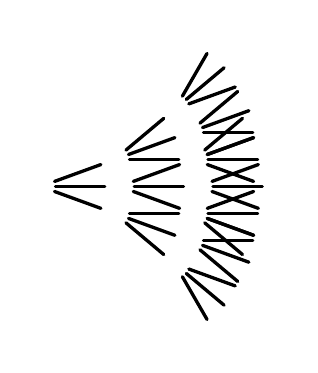
\begin{tikzpicture}[grow cyclic, shape=circle, level distance=10mm, very thick, cap=round]
\node [color=green] {} 
    child { node {}
        child { node {} 
            child { node {} }
            child { node {} }
            child { node {} }
        }
        child { node {} 
            child { node {} }
            child { node {} }
            child { node {} }
        }
        child { node {} 
            child { node {} }
            child { node {} }
            child { node {} }
        }
    }
    child { node {}
        child { node {} 
            child { node {} }
            child { node {} }
            child { node {} }
        }
        child { node {} 
            child { node {} }
            child { node {} }
            child { node {} }
        }
        child { node {} 
            child { node {} }
            child { node {} }
            child { node {} }
        }
    }
    child { node {}
        child { node {} 
            child { node {} }
            child { node {} }
            child { node {} }
        }
        child { node {} 
            child { node {} }
            child { node {} }
            child { node {} }
        }
        child { node {} 
            child { node {} }
            child { node {} }
            child { node [color=red] {} }
        }
    };
\end{tikzpicture}
\caption{All possible states from a planning problem with 3 actions applied 3 times from the initial state (green). Possible solution marked as red.}
\end{figure}

A typical example is the classical \emph{blocks world} domain where there are three blocks ($A,B$ and $C$) that can be piled   on a table. The possible actions are picking blocks and letting blocks on top of a block or on the table. These actions have preconditions forbidding their executions (for instance a block that is under another block can not be picked) and effects that change the state of the world. A particular instance of the problem consists on a configuration of the blocks, for example, $A$ is on top of $B$ which is on top of $C$ which is on the table, and a desired goal state, for example, $C$ is on top of $B$ which is on top of $A$ which is on the table. For this particular problem a possible plan would be these consecutive actions: pick $A$ and let it on the table, pick $B$ and let it on $A$ and pick $C$ and let it on $B$.


\section{Planning Domain Definition Language}
The Planning Domain Definition Language (PDDL)~\cite{pddl1.2,pddl2.1,pddl2.2,pddl3.0,pddl3.1,pddl3.1-corrected} is a standard Artificial Intelligence planning language. It's the official language for the International Planning Competition (IPC)~\cite{icaps}, which has evolved with each competition. The current PDDL version is the 3.1~\cite{pddl3.1-corrected}.

The language separates the domain description and the (particular instance) problem description. The domain defines all possible actions from a plan, while the problem defines the initial state and possible goal states. An example can be seen in Example~\ref{ex:pddl}.

\vspace{1\baselineskip}

\begin{example}
\label{ex:pddl}
Problem example where a robot has to move the ball \textit{1} from room \textit{A} to room \textit{B}. The problem contains the following actions:
\begin{description}
    \item[move (?from ?to)] move the robot from the room \textit{?from} to the room \textit{?to} 
    \item[pick (?obj ?room ?gripper)] pick an  object \textit{?obj} with the arm \textit{?gripper} which is in the room \textit{?room}
    \item[drop (?obj ?room ?gripper)] drop an object \textit{?obj} from the arm \textit{?gripper} to the room \textit{?room}
\end{description}

\vspace{1\baselineskip}

The problem uses the following predicates:
\begin{description}
    \item[(room ?r)] true if the object \textit{?b} is a room
    \item[(ball ?b)] true if the object \textit{?b} is a ball
    \item[(gripper ?g)] true if the object \textit{?b} is an arm
    \item[(at-robby ?r)] true if the robot is in the room \textit{?r}
    \item[(at ?b ?r)] true if the object \textit{?b} is in the room \textit{?r}
    \item[(free ?g)] true if the ram \textit{?g} is not carrying anything
    \item[(carry ?o ?g)] true if the object \textit{?o} is been carried by the arm \textit{?g}
\end{description}

\vspace{1\baselineskip}

Note that the action parameters can be instantiated by any object, for example in the action \textit{move}, the parameter \textit{?from} can be instantiated the object \textit{rooma} but also can be the object \textit{left}. To restrict only the rooms to be valid, the predicate \textit{(room ?r)} is needed.

The domain description:
\begin{lstlisting}
(define (domain gripper-strips)
   (:predicates (room ?r)
        (ball ?b)
        (gripper ?g)
        (at-robby ?r)
        (at ?b ?r)
        (free ?g)
        (carry ?o ?g))

   (:action move
       :parameters (?from ?to)
       :precondition (and (room ?from) (room ?to) (at-robby ?from))
       :effect (and (at-robby ?to)
             (not (at-robby ?from))))

   (:action pick
       :parameters (?obj ?room ?gripper)
       :precondition (and (ball ?obj) (room ?room) (gripper ?gripper)
                (at ?obj ?room) (at-robby ?room) (free ?gripper))
       :effect (and (carry ?obj ?gripper)
            (not (at ?obj ?room)) 
            (not (free ?gripper))))

   (:action drop
       :parameters (?obj ?room ?gripper)
       :precondition (and (ball ?obj) (room ?room) (gripper ?gripper)
                (carry ?obj ?gripper) (at-robby ?room))
       :effect (and (at ?obj ?room)
            (free ?gripper)
            (not (carry ?obj ?gripper)))))
\end{lstlisting}

Predicates are initialized inside the block \textit{init}, i.e., \textit{(:init (room rooma))} initializes the predicate \textit{room} with the object \textit{rooma} to true.

The problem definition with the initial state and the goal restrictions:
\begin{lstlisting}
(define (problem strips-gripper2)
    (:domain gripper-strips)
    (:objects rooma roomb ball1 ball2 left right)
    (:init (room rooma)
           (room roomb)
           (ball ball1)
           (ball ball2)
           (gripper left)
           (gripper right)
           (at-robby rooma)
           (free left)
           (free right)
           (at ball1 rooma)
           (at ball2 rooma))
    (:goal (at ball1 roomb)))
\end{lstlisting}
\end{example}

\subsection{Subset adl}
The \emph{adl} subset is one of the most basic PDDL language subsets using:
\begin{itemize}
    \item strips: STRIPS language-like planning problem definition (see~\cite{wiki:strips} for further STRIPS details)
    \item typing: Group objects into types
    \item negative-preconditions: Use of \emph{not} predicate in preconditions
    \item equality: Equality between objects
    \item quantified-preconditions: Use of \emph{forall} and \emph{exists} in preconditions. The language uses a closed-world assumption
    \item conditional-effects: Use of \emph{when} predicate in effects
\end{itemize}

Since any problem can be described only using \emph{strips}, \emph{adl} facilitates the language syntax.

\subsection{Subset numeric-fluents}
The \emph{numeric-fluents} subset allows a new kind of predicates named \emph{function} which can return an integer number.

\subsection{Subset object-fluents}
The \emph{object-fluents} subset is the latest language subset which allows the functions to return objects instead of the integer number type. This allows the language to be more expressive.

\section{Planner}
A planner is a domain-independent software which aims to solve a planning problem. Usually the input is a PDDL-model, composed by the domain and the problem.

\section{Boolean Formulas}

Given a set {\tt X} of Boolean variables, a Boolean formula {\tt F} can be constructed by the grammar:
\begin{center}
\begin{verbatim}
    F ::= X
       |  not F
       |  F \/ F
       |  F /\ F
       |  F -> F
       | ( F )
\end{verbatim}
\end{center}
where disjunction ($\vee$) and conjunction ($\wedge$) operators are associative.
Further operators exist but do not add further complexity. Moreover, all formulas can be equivalently expressed using just the negation ($\neg$), disjunction and conjunction  operators since, in fact, $A\to B$ is equivalent to $\neg A \vee B$.

\section{Propositional satisfiability problem}
An interpretation is an assignment (or mapping) of truth values (true or false) to Boolean variables. 

The propositional satisfiability problem (SAT) is the well known problem of determining, if given a Boolean formula, there exists any interpretation that satisfies it. In other words, if all variables can be replaced by their assigned truth values and the formula evaluates to \textit{true}.

\vspace{1\baselineskip}

\begin{example} An example of a  SAT problem.
\begin{align*}
& (\lnot A \vee \lnot B \vee \lnot C) \quad \wedge \\
& (A \vee \lnot C) \quad \wedge \\
& (\lnot B \vee E \vee \lnot E) \quad \wedge \\
& (C)
\end{align*}

A possible interpretation satisfying the formula could be $\{A, \lnot B, C, D , E\}$.
\end{example}

SAT has been proven to be NP-complete, which means that all problems in the class NP are at most as difficult to solve as SAT.

\section{SAT Modulo Theories}
The satisfiability modulo theories (SMT) problem is a decision problem for logical formulas with respect to a background theory, for example the theory of integers. It can be though as a form of SAT where instead of having just Boolean variables or their negations as literals, it can also have atoms that will be evaluated to true or false according to some background theories, e.g., $(x<2+y)$, where the predicate $<$ is comparing two arithmetic expressions containing integer variables $x$ and $y$. See~\cite{smt} for further details.

The SMT-LIB is a library and set of standards for SMT systems, which includes a language. The latest language version is the \emph{2.6}.

Possible \emph{SMT-LIB 2.0} Logical operators are:
\begin{itemize}
    \item main logical operations: (and), (or), (xor), (not)
    \item implication (=\textgreater), equality (=) and distinction (distinct)
    \item it-then-else (ite)
\end{itemize}

In addition, the \emph{Ints} theory allow the following operations:
\begin{itemize}
    \item addition (+) and substraction (-)
    \item multiplication (*), division (div) and modulo (mod)
    \item absolute value (abs)
    \item smaller than (\textless), smaller or equal than (\textless=), larger than (\textgreater), larger or equal than (\textgreater=)
\end{itemize}

\vspace{1\baselineskip}

\begin{example} An SMT problem using \emph{SMT-LIB 2.0} and \emph{Ints} theory with Linear Integer Arithmetic (LIA) logics:
\begin{lstlisting}
(set-logic QF_LIA)
(declare-const x Int)
(declare-const y Int)
(declare-const a Bool)
(assert (= a true))
(assert (and (= (- x y) (+ x (- y) 1)) a))
(check-sat)
(exit)
\end{lstlisting}

The result is unsat, meaning there isn't an interpretation, or a possible assignment which satisfies the conjunction of the formulas:
\begin{gather}
a \leftrightarrow true \\
x - y = (x + (-y) + 1) \quad \wedge \quad a
\end{gather}
\end{example}

\section{Planning as Satisfiability}
Planning as Satisfiability is a planning resolution technique based in reducing the problem to SAT by encoding as a Boolean formula the question ``is there a sequence of $n$ actions that brings from state $S^0$ to a final state?''. In other words, it consists in, for a given number of steps $n$, defining $n+1$ possible states (being $S^0$ the initial state and $S^n$ the final one) and choosing $n$ actions to perform these transitions from state to state. The initial state variables are initialized by the encoding using the instance, meanwhile the other states variables will be resolved by the SAT solver.

The encoding must ensure that the chosen action at time step $t$ can be performed, since its precondition is met at state $S^t$ and it must also ensure that their effects are applied at state $S^{t+1}$. Moreover, the encoding has also to ensure that only one action is chosen and that variables not involved in the effect of the chosen action do not ``freely'' change from one state to the other.

\begin{figure}[h]
\centering
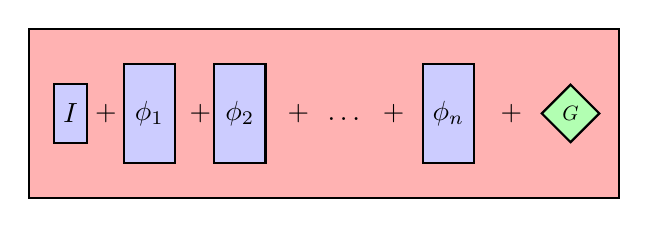
\begin{tikzpicture}[auto, thick]
\node [thick, rectangle, minimum width=4.5cm, minimum
height=2cm] (check) at (0,0) {  };  

\node [draw, thick,rectangle, minimum width=7.5cm, fill=red!30,minimum
height=2.15cm] (check2) at ([shift={(1.44,0)}]check) {  };  

\node [thick, rectangle, minimum width=3cm, minimum height=1.875cm] (check2) at ([shift={(-.68,0)}]check) {  };  

\node [ thick, rectangle, minimum width=1.75cm, minimum
height=1.75cm, ] (check3) at ([shift={(-.55,0)}]check2) {  };  

\node [draw, fill=blue!20,thick, rectangle,minimum width=.25cm, minimum
height=.75cm] (inici) at ([shift={(-1.1,0)}]check2) { $I$ };  

\node [] at ([shift={(.45,0)}]inici) { + };
\node [draw, thick, fill= blue!20,rectangle,minimum width=.65cm, minimum
height=1.25cm] at ([shift={(1,0)}]inici) { $\phi_1$ };  
\node [] at ([shift={(1.65,0)}]inici) { + };
\node [draw, thick, fill= blue!20,rectangle,minimum width=.65cm, minimum
height=1.25cm] at ([shift={(2.15,0)}]inici) { $\phi_2$ };
\node [] at ([shift={(3.5,0)}]inici) { +\ \ \dots\ \ + };  
\node [draw, thick, fill= blue!20,rectangle,minimum width=.65cm, minimum
height=1.25cm] (phin) at ([shift={(4.8,0)}]inici)  { $\phi_n$ };  

\node [] at ([shift={(5.6,0)}]inici) { + };
\node [draw,thick, fill= green!30,diamond,minimum width=.5cm,scale=.75] at
([shift={(6.35,0)}]inici)  {$G$};
\end{tikzpicture}
\caption{SAT formula encoding plan feasibility  if $n$ time-steps. $I$ are $S^0$ assignments, $\phi_i$s are formulas encoding sound transition between states according to a chosen action for the $i$-th time-step and $G$ are the goal state restrictions.}\label{fig:steps}
\end{figure}

It is important to highlight that an encoding of $n$ time steps encodes a planning problem of exactly $n$ actions. To check if there exists a plan for $n$ or fewer actions, it is needed to generate and solve $n$ different encodings, each one with a one more time step than the previous one. Figure~\ref{fig:steps} illustrates the formula for $n$ time-steps.

When the problem to model requires, for instance, integer variables to represent the state, it makes sense to consider planning as satisfiability modulo theories instead of just planning as satisfiability (see for instance~\cite{rantanplan}).

\chapter{System requirements}
The system requirements can be split into functional and nonfunctional requirements.

\section{Functional requirements}
The Snowman editor functional requirements are the followings:
\begin{itemize}
    \item The user must be able to create a custom level
    \item The user must be able to play the level
    \item The user must be able to save the level
    \item The user must be able to load a level
    \item The user must be able get the optimal solution to a level
    \item The user must be able to get an approximate solution to a level
\end{itemize}

\section{Nonfunctional requirements}
To run the Snowman Editor the following requirements must be satisfied:

\subsubsection{Hardware requirements}
\begin{description}
    \item[OS:] Any \emph{Linux} distribution (64 bits). \emph{Windows} \footnote{Windows seems to have performance issues with \emph{Yices 2}} and \emph{Mac OS X} are also supported but not tested.
    \item[CPU:] Any. It is recommended to have a good single thread performance.
    \item[RAM:] 16 GB. It is recommended to have high speed and low latency ram.
\end{description}

\subsubsection{Software requirements}
\begin{itemize}
    \item \emph{Yices 2}. Tested with version 2.5.4
    \item \emph{A Good Snowman Is Hard To Build}. Tested with the Steam content BuildID 1086215
    \item \emph{Java SE Runtime Environment 8}
    \item \emph{Java Development Kit 8}
\end{itemize}

\chapter{Studies and decisions}
This chapter describes all the studies and decisions that have been made during the development of this project.

\section{PDDL as a problem description language}
Instead of performing an ad hoc approach to the \emph{Snowman problem}, an alternative is to use existing software that solves generic planning problems by defining the problem as an input. The most used and updated planning description language is  PDDL.

\section{Scala as a programming language}
\emph{Scala} has been chosen to be the main developing language because, like \empty{Java}, it is an operative system independent language. Also its functional approach allows for a more clear, simple to write, code.

\section{Functional programming}
Most of this project's code follows the functional program paradigm. There are some cases where imperative programming was added to improve performance or to simplify the code structure. Since this project does not have a big parallelism component, the functional programming is not mandatory and the main reason it has been chosen is to explore this paradigm.

\section{SMT versus SAT}
To facilitate the encoding programming, the problem is encoded in SMT instead of SAT. This allows the use of Integer theory and avoids its codification to SAT. Anyway, a translation from SMT to SAT is possible and should be as simple as implementing a SAT \emph{translator}.

\section{Yices 2 as an SMT Solver}
\emph{Yices 2}\cite{yices2,yices} is an open source \emph{SMT} solver which can process input written in the \emph{SMT-LIB} notation. It has been chosen because, according to the knowledge of the group where I'm developing the project, it is one of the best solvers that supports \emph{SMT-LIB 2.0}. However, it should not be difficult to use any other SMT solver also supporting \emph{SMT-LIB 2.0}.

\chapter{Analysis and Design}
This chapter describes the all work done and its details.

\section{Snowman Editor}
The \emph{Snowman Editor} is a software package which includes all the work done in this project. This software allows to edit, play and solve \emph{Snowman problem} instances. The software code is split in four modules each one encapsulating a different functionality.
\begin{itemize}
    \item Planner module
    \item Snowman problem module
    \item Game modification module
    \item GUI module
\end{itemize}

Because the code contains more than a hundred classes, without including the companion objects for some of these classes, the following analysis only focuses on the more interesting parts. 

\subsection{Planner module}
The \emph{planner} module (package \emph{planner}) is an abstraction of a planning as satisfiability solver. By giving a custom \emph{encoder}, \emph{translator} and \emph{solver}, it will search for a plan. The pipeline can be seen in Figure~\ref{fig:pipeline}. A complete class diagram can be seen in Figure~\ref{fig:planner-class-diagram}.

\begin{figure}
    \smartdiagramset{uniform color list=white for 10 items, uniform arrow color=true, arrow color=black, back arrow disabled=true, 
        additions={
            additional item offset=0.6cm,
            additional arrow color=black,
        }
    }
    
    \smartdiagramadd[flow diagram:horizontal]{Instance, \textit{Encoder}, Internal language, \textit{Translator}}{right of module4/ }
    \smartdiagramconnect{->}{module4/additional-module1}
    
    \vspace{1\baselineskip}
    
    \begin{center}
    \hspace*{\fill} \smartdiagramadd[flow diagram:horizontal]{Planner, Timestep solver, \textit{Solver}, Plan}{left of module1/ }
    \smartdiagramconnect{->}{additional-module1/module1}
    \end{center}
    
    \vspace{1\baselineskip}

    \caption{The planner pipeline}
    \label{fig:pipeline}
\end{figure}

\vspace{1\baselineskip}

The \emph{planner} uses an abstract \emph{internal language} similar to \emph{SMT-LIB}. The parse tree (Figure~\ref{fig:parse-tree}) is represented by classes subclassing, but because of the Scala language limitations, a more generic parsing tree (Figure~\ref{fig:parse-tree-generic}) has been used, but checking the types during run-time.

\begin{figure}
    \centering
    \begin{verbatim}
    Expressison -> expression (ClauseDeclaration | VariavleDeclaration | Comment)
    ClauseDeclaration -> clauseDeclaration Clause
    VariavleDeclaration -> variableDeclaration Clause
    Comment -> comment [Scala String]
    Clause -> clause (Add | Or | Not | Implies | Equivalent | BooleanVariable |
        BooleanConstant | Add | Sub | Equals | Smaller | Greater | 
        IntegerVariable | IntegerConstant)
    And -> and Clause Clause
    Or -> or Clause Clause
    Not -> not Clause
    Implies -> implies Clause Clause
    Equivalent -> equivalent Clause Clause
    BooleanVariable -> booleanVariable [Scala Boolean]
    BooleanConstant -> booleanConstant [Scala Boolean]
    Add -> add Clause Clause
    Sub -> sub Clause Clause
    Equal -> equal Clause Clause
    Smaller -> smaller Clause Clause
    Greater -> greater Clause Clause
    IntegerVariable -> integerVariable [Scala Int]
    IntegerConstant -> integerConstant [Scala Int]
    \end{verbatim}
    \caption{\emph{Internal language} generic parse tree}
    \label{fig:parse-tree-generic}
\end{figure}

\begin{figure}
    \centering
    \begin{verbatim}
    Expressison -> expression (ClauseDeclaration | VariavleDeclaration | Comment)
    ClauseDeclaration -> clauseDeclaration (BooleanClause | IntegerClause)
    VariavleDeclaration ->  variableDeclaration (BooleanVariable | IntegerVariable)
    Comment -> comment [Scala String] 
    BooleanClause -> booleanClause (Add | Or | Not | Implies | Equivalent | Smaller |
        Greater | Equals)
    IntegerClause -> integerClause (Add | Sub | IntegerVariable | IntegerConstant)
    And -> and BooleanClause BooleanClause
    Or -> or BooleanClause BooleanClause
    Not -> not BooleanClause
    Implies -> implies BooleanClause BooleanClause
    Equivalent -> equivalent BooleanClause BooleanClause
    BooleanVariable -> booleanVariable [Scala Boolean]
    BooleanConstant -> booleanConstant [Scala Boolean]
    Add -> add IntegerClause IntegerClause
    Sub -> sub IntegerClause IntegerClause
    Equal -> equal IntegerClause IntegerClause
    Smaller -> smaller IntegerClause IntegerClause
    Greater -> greater IntegerClause IntegerClause
    IntegerVariable -> integerVariable [Scala Int]
    IntegerConstant -> integerConstant [Scala Int]
    \end{verbatim}
    \caption{\emph{Internal language} parse tree}
    \label{fig:parse-tree}
\end{figure}

\vspace{1\baselineskip}

\begin{example} 
Scala code examples as an abstraction of the \emph{Internal language}:
\begin{lstlisting}
And(Equals(b.x, bNext.x), Equals(b.y, bNext.y), Equals(b.size, bNext.size))
Smaller(stateNext.mediumBalls, IntegerConstant(2 * level.snowmans + 1))
Equivalent(eff, actionVariable)
\end{lstlisting}
\end{example}

\subsubsection{Encoder}
The \emph{encoder} is an abstraction (Figure~\ref{fig:encoder-interface}) which defines encoding of the problem instance to the \emph{internal language}. Also is responsible to translate the \emph{solver} result to \emph{planner} actions. 

\begin{figure}
    \centering
    \includegraphics[scale=0.25]{encoder-interface.png}
    \caption{Encoder interface}
    \label{fig:encoder-interface}
\end{figure}

\subsubsection{Translator}
The \emph{translator} is an abstraction (Figure~\ref{fig:translator-interface}) which defines the translation of the the internal \empty{language} to the \emph{solver} language. The solver language is a generic type which is defined by the solver.

\begin{figure}
    \centering
    \includegraphics[scale=0.25]{translator-interface.png}
    \caption{Translator interface}
    \label{fig:translator-interface}
\end{figure}

\subsubsection{Solver}
The \emph{solver} an abstraction (Figure~\ref{fig:solver-interface}) which defines the interface between the planner and the external solver. It inputs the \emph{translator} result to the solver and passes the output to the \emph{encoder} to decode. 

\begin{figure}
    \centering
    \includegraphics[scale=0.25]{solver-interface.png}
    \caption{Solver abstract class}
    \label{fig:solver-interface}
\end{figure}

\subsubsection{Planner submodule and Timestep solver}
The \emph{Planner submodule} is the main solver sub-module which launches multiple \emph{Timestep solvers} in parallel or sequentially. Meanwhile, the \emph{Timestep solver} is a sub-module which solves an encoding of $n$ time steps. The planner will launch different \emph{Timestep solvers}, with an increasing formula of $n$ time steps, until a solution is found.

The planner is able to use parallelism by launching multiple \emph{Timestep solvers} at the same time, each one with an encoding for a different number of time steps. If a solution is found in $n$ time steps, it will kill all the executions with a bigger time step and will finish the lower time step encoding already running. Once all of them are finished, will pick the solution with the lower time step as the final solution.

Using a single machine (with 4 cores and hyperthreading), the best performance seems to be using 3 threads (Figure~\ref{fig:threads}), this can be caused by the cache sharing since the SAT/SMT solvers usually are memory dependent.

\begin{figure}
    \begin{center}
    \begin{tabular}{||c|c|c||}
        \hline
        \textbf{Cores} & \textbf{Time (s)} & \textbf{Ratio} \\
        \hline\hline
        1 & 345754 & 1 \\
        \hline
        2 & 201991 & 1.712 \\
        \hline
        3 & 165163 & 2.083 \\
        \hline
        4 & 168111 & 2.057 \\
        \hline
        5 & 181119 & 1.909 \\
        \hline
        6 & 199880 & 1.730 \\
        \hline
        7 & 203140 & 1.702 \\
        \hline
        8 & 224669 & 1.539 \\
        \hline
    \end{tabular}  
    \end{center}
    \caption{Time results solving the Sarah level using the \textit{Basic encoding}}
    \label{fig:threads}
\end{figure}

\begin{figure}
    \centering
    \includegraphics[width=\textwidth,height=0.93\textheight,keepaspectratio]{planner-class-diagram.png}
    \caption{Class diagram from the planner module}
    \label{fig:planner-class-diagram}
\end{figure}

\subsubsection{Packages}
Description of the packages found in this module.
\begin{description}
    \item[\emph{encoder}] Encoder abstraction interfices. A complete class diagram can be seen in Figure~\ref{fig:snowman-encoder-class-diagram}
    \item[\emph{operations}] \emph{Internal language} parse tree definition, run-time checks and utilities
    \item[\emph{planner}] Main functions for the planner
    \item[\emph{solver}] Solver abstraction interfices
    \item[\emph{timestep}] Single formula encoding solver
    \item[\emph{translator}] Translator interfices
\end{description}

\subsection{Snowman problem module}
The \emph{snowman problem} module (package \emph{snowman}) is the concrete implementation of the planning problem. It implements all the abstractions needed by the \emph{planner}. Also it is responsible of generation the \emph{PDDL problem} given an instance.

Also this module includes all the data structures to represent a game level and its properties. 

The module contains one \emph{encoder} for each of the three encodings. To avoid code repetition between the three encoders, a generic Template (figure \ref{fig:template}) pattern has been used in the encoder classes, while a Strategy pattern has been used with the states attributes. Also, the encoders are instantiated using a Factory in the \textit{BaseEncoder} object.

\begin{figure}
    \centering
    \includegraphics[scale=0.25]{template-class-diagram.png}
    \caption{Generic template class diagram}
    \label{fig:template}
\end{figure}

\newpage

\subsubsection{Packages}
Description of the pacakges found in this module.
\begin{description}
    \item[\emph{action}] Actions the snowman planning problem can perform
    \item[\emph{collection}] Custom collections
    \item[\emph{encoder}] Concrete \emph{planner} encoder implementation. Contains all the encodings
    \item[\emph{game}] Game constants and description
    \item[\emph{level}] Level data structure
    \item[\emph{pddl}] PDDL instances generator
    \item[\emph{planner}] Submodule which interfaces with the planner module
    \item[\emph{solver}] Concrete \emph{planner} solver implementation
    \item[\emph{translator}] Concrete \emph{planner} translator implementation
    \item[\emph{util}] Various utilities
    \item[\emph{validator}] Planning validator
\end{description}

\begin{figure}
    \centering
    \includegraphics[width=\textwidth,height=0.93\textheight,keepaspectratio]{snowman-encoder-class-diagram.png}
    \caption{Class diagram from the planner planner package from Snowman problem module}
    \label{fig:snowman-encoder-class-diagram}
\end{figure}

\subsection{Game modification module}
The \emph{game modification} module (package \emph{mod}) is in charge of altering the game files to launch the game with a custom level. Also, it allows to restore the game to the previous state. A custom levels is being loaded by altering multiple resources files and the save game files.

\subsection{GUI module}
Finally, the \emph{GUI} module (package \emph{ui}) is the level editor, but also the main module which calls all the other modules. The \emph{GUI} is written in a native way using \emph{Scala/Java Swing}.

This module is completely independent from the other modules which allows to change the graphical interface without any code modification.

\begin{figure}
    \begin{center}
    \includegraphics[scale=0.3,valign=t]{gui-module-1.png}
    \includegraphics[scale=0.3,valign=t]{gui-module-2.png}
    \end{center}
    \caption{Some screenshots examples from the graphical interface}
    \label{fig:gui-module}
\end{figure}

\section{PDDL Approach}
The PDDL approach aims to solve the \emph{Snowman problem} by using the PDDL standard Artificial Intelligence planning language. Because of the limitations with PDDL and its planers, two different approaches have been taken. 

\subsection{\emph{adl} approach}
The main idea behind the \emph{adl} approach is to associate a distinct object to each possible locations of the level at hand, and to use predicates to define the adjacencies between them, i.e., the object \textit{loc-1-1} represents the level coordinate $1,1$. The predicates are:

\begin{description}
    \item[(snow ?l - location)] Is true if location \textit{?l} has snow
    \item[(next ?from ?to - location ?dir - direction)] Is true if locations \textit{?from} and \textit{?to} are adjacents and align in the direction \textit{?dir}
    \item[(occupancy ?l - location)] Is true if a location \textit{?l} is occupied by a ball
    \item[(character-at ?l - location)] Is true if the character is at location \textit{?l}
    \item[(ball-at ?b - ball ?l - location)] Is true if a ball \textit{?b} is at location \textit{?l}
    \item[(ball-size-small ?b - ball)] Is true if the ball \textit{?b} size is small
    \item[(ball-size-medium ?b - ball)] Is true if the ball \textit{?b} size is medium
    \item[(ball-size-large ?b - ball)] Is true if the ball \textit{?b} size is large
    \item[(goal)] Is true if all the goal restrictions are meet
\end{description}

There are only two actions but the action \emph{move\_ball} uses \emph{conditional-effects}:
\begin{description}
    \item[move\_character (?from ?to - location ?dir - direction] Move the character from location \textit{?from} to location \textit{?to} and both locations are align in the direction \textit{?dir}
    \item[move\_ball (?b - ball ?ppos ?from ?to - location ?dir - direction)] Move the ball from location \textit{?from} to location \textit{?to} if the player is at the location \textit{?ppos} and all three locations are align in the directoin \textit{?dir}. Update the snow, ball size and move the character according to the game rules.
\end{description}

The predicate occupancy is used to check if the character can be moved to its destination.

The \emph{conditional-effects} could be removed by unfolding each conditional effect in a new action with the conditional statement as a new predicate and the effect as main effect.

\subsubsection{The \emph{move\_ball} action}
Here follows the \emph{move\_ball} action  definition:

\paragraph{Precondition}
Description of the different statements used in the precondition:

Locations must be aligned.
\begin{lstlisting}
(next ?ppos ?from ?dir)
(next ?from ?to ?dir)
\end{lstlisting}

The character must be behind the ball. Encodes the game rule number 1.
\begin{lstlisting}
(ball-at ?b ?from)
(character-at ?ppos)
\end{lstlisting}

All the balls being at the same location as the ball which is being moved must be bigger. Encodes the rule number 4.
\begin{lstlisting}
(forall (?o - ball)
    (or 
        (= ?o ?b)
        (or 
            (not (ball-at ?o ?from))
            (or 
                (and
                    (ball-size-small ?b)
                    (ball-size-medium ?o))
                (and
                    (ball-size-small ?b)
                    (ball-size-large ?o))
                (and
                    (ball-size-medium ?b)
                    (ball-size-large ?o))))))
\end{lstlisting}

If there is a ball at the same location as the ball which is being moved, it can not be a ball in front. Encodes the rule number 3 and 4.
\begin{lstlisting}
(or
    (forall (?o - ball)
        (or 
            (= ?o ?b)
            (not (ball-at ?o ?from))))
    (forall (?o - ball)
            (not (ball-at ?o ?to))))
\end{lstlisting}

If there is a ball in front of the ball which is being moved, it has to be larger. Encodes the rule number 4.
\begin{lstlisting}
(forall (?o - ball)
    (or
        (not (ball-at ?o ?to))
        (or 
            (and
                (ball-size-small ?b)
                (ball-size-medium ?o))
            (and
                (ball-size-small ?b)
                (ball-size-large ?o))
            (and
                (ball-size-medium ?b)
                (ball-size-large ?o))))))
\end{lstlisting}

\vspace{1\baselineskip}

Notice that the structure \textit{(or (not (A)) (B))} is a logical implication.

\paragraph{Effect}
Description of the different statements used in the effect:

The goal is true if all the balls are at the same location.
\begin{lstlisting}
(when
    (forall (?o - ball)
        (or (= ?o ?b)
        (ball-at ?o ?to)))
    (goal))
\end{lstlisting}

Update the occupancy predicate according to the ball movement.
\begin{lstlisting}
(not (occupancy ?from))
(occupancy ?to)
\end{lstlisting}

Update the ball location.
\begin{lstlisting}
(not (ball-at ?b ?from))
(ball-at ?b ?to)
\end{lstlisting}

Move the character to the new location only if there was no ball under.
\begin{lstlisting}
(when
    (forall (?o - ball)
        (or 
            (= ?o ?b)
            (not (ball-at ?o ?from))))
    (and
        (not (character-at ?ppos))
        (character-at ?from)))
\end{lstlisting}

It removes the snow. It is always removed.
\begin{lstlisting}
(not (snow ?to))
\end{lstlisting}

If there was snow, it increases the ball size.
\begin{lstlisting}
(when
    (and
        (snow ?to)
        (ball-size-small ?b))
    (and
        (not (ball-size-small ?b))
        (ball-size-medium ?b)))
(when
    (and
        (snow ?to)
        (ball-size-medium ?b))
    (and
        (not (ball-size-medium ?b))
        (ball-size-large ?b))))
\end{lstlisting}

The full \emph{adl} PDDL model can be found in Appendix \ref{annex:pddl-adl}.

An unfolded action can be seen as generating a new action for every combination parameters, referencing the concrete object when the parameter is being used. The main problem with this approach is the number of unfolded action which, because is to large, makes the search impossible. For example, the Andy instance, one of the smallest instances, has 3 balls and 25 playable locations. The number of unfolded actions would be:
\begin{description}
    \item[move\_character (?from ?to - location ?dir - direction)] $25\ (?from) * 25\ (?to) * 4\ (?dir) = 2500$
    \item[move\_ball (?b - ball)] $3\ (?ball) * 25\ (?ppos) * 25\ (?from) * 25\ (?to) * 4\ (?dir) = 187500$
\end{description}
In total $190000$ actions to explore every state, in contrast of the 4 actions the game has.

Another possible approach would substitute all the parameters by \emph{conditional-effects}, but this approach is not possible since PDDL does not support nested  \emph{conditional-effects}.

\subsection{object-fluents approach}
The \emph{object-fluents} approach aims to reduce the number of actions by removing all the location and directions from the action parameters. They can be removed because a new set of functions which saves the character and ball locations are introduced. Also, a new set of \emph{next} functions are introduced which acts like the old \emph{next} predicate. The new functions are:
\begin{description}
    \item[(character-at) - location] Returns the object location which is the character
    \item[(ball-at ?b - ball) - location] Returns the object location which is the ball \textit{?b}
    \item[(next-up ?l - location) - location] Returns the object location which is in from of location \textit{?l}
    \item[(next-down ?l - location) - location] Returns the object location which is behind of location \textit{?l}
    \item[(next-right ?l - location) - location] Returns the object location which is in to right of location \textit{?l}
    \item[(next-left ?l - location) - location] Returns the object location which is in to left of location \textit{?l}
\end{description}

\vspace{1\baselineskip}

Because the direction is removed from the action parameter, now there will be 4 actions of each kind, one for each direction. The number of unfolded actions for the Andy instance becomes just $16$:
\begin{description}
    \item[move character] $4\ actions$
    \item[move\_ball (?b - ball ?ppos ?from ?to - location ?dir - direction)] $4\ actions * 3\ (?ball) = 12$
\end{description}

\vspace{1\baselineskip}

The full \emph{object-fluents} PDDL model can be found in Appendix \ref{annex:pddl-object-fluents}.

The main problem of this description is that the only planner that supports this subset is \emph{Rantanplan}\cite{rantanplan}. This planner uses planning as SMT approach and supports this PDDL specification. However the initial experiments with a basic configuration have been quite disappointing since it was not able to solve the simplest game  instance. Further configurations of the solver should be considered to try to solve real instances. This is left as further work.

\subsection{Using a planner to solve the problem: The reality}
Once the domain and the problem descriptions are generated, they can be used as input to a planner. Multiple planners from the last \emph{IPC} (2018) have been tested but none of them could solve a single instance. Most of the planners were based on the planner \emph{Fast Downward}\cite{fastdownward}, which seems to have a problem interpreting the \emph{Snowman problem} domain, which makes the planner to not halt. Other planners simply did return an invalid plan.

Because searching for newer planners is a very time consuming task, this part (and possible results) has been left as further work.

\section{SMT Approach}
The SMT approach allows to find an optimal solution to the \emph{Snowman problem}. This is desired since the main objective of the project is to find undesired solutions, which usually are easier solutions that the wanted solution.

During the encoding development process three different encodings have been created since each one has its advantages an inconveniences. The theory used is Linear Integer Arithmetic since integer variables and linear arithmetic expressions are required.

\subsection{Basic encoding: The first SMT encoding}
A first approach to encode the \emph{Snowman problem} is to encode all possible actions a player can do in the game. Even though there are only four actions in the game (up, down, left, right)\footnote{The game is played using the keyboard arrows}, since they have different effects, these actions can be split into two categories: character movement actions and ball movement actions.

This way, this first encoding encodes four actions for the character movement actions and four actions for the ball movement actions, but for each ball. To perform a ball movement action, first the player has to travel next to the ball using the character movements actions. Example~\ref{ex:tanya-basic} shows the solution found for the Tanya problem with the \emph{Basic encoding}.

The preliminary result hovever, showed that this first encoding was not able to solve many levels in a reasonable time.

\subsubsection{Instance}
Each problem instance has the following information:
\begin{itemize}
    \item Set of locations of the scenario: $Pos$.
    \item Initial character location: $Character$. 
    \item Set of balls with their initial locations and sizes: $Balls$.
    \item Set of initial floor locations with snow: $Snow$.
    \item Set of wall locations: $Walls$.
\end{itemize}

A location is a coordinate, i.e., a pair of natural numbers $(x,y)$.

For the sake of readability of the following encoding, the set $BallPos$ is defined as $(i,j)\in Pos$ such that there exists $b \in Balls$ with  $b.x = i \wedge b.y = j$.

\subsubsection{State}
The game state at time step $t$ will be represented by the following state variables $\langle c, b, s, o, ibs\rangle$:
\begin{itemize}
\item Character coordinates variables. Integer variables for each time step $t$: $c^t.x$ and $c^t.y$.
\item Set of ball variables. Integer variables for each time step $t$ and ball $k$: $b_k^t.x, b_k^t.y$ and $b_k^t.size$ 
\item Set of snow variables that represent if each coordinate has snow. Boolean variables for each time step $t$, and coordinates $x,y$: $s_{x,y}^t$
\item Set of occupancy variables that represent if there's a ball or a wall. Boolean variables for each time step $t$, and coordinates $x,y$: $o_{x,y}^t$
\item For the invariant \textit{INVARIANT\_BALL\_SIZES}, and if the invariant is enabled, for each time step $t$, a medium size balls counter $ibs_m^t$ and a large size balls counter $ibs_l^t$
\end{itemize}

A state $S^t$ will be a valuation over the sets of state variables of time step $t$.

\subsubsection{Initial state}
In the encoding the initial state is defined, according to the instance data, by the following formula, see Example~\ref{ex:s0}
\begin{gather*}
c^0.x = Character.x \quad \wedge \quad c^0.y = Character.y \\
\bigwedge \limits_{k \in Balls} (b_k^0.x = Balls_k.x \quad \wedge \quad b_k^0.y = Balls_k.y \quad \wedge \quad b_k^0.size = Balls_k.size) \\
\bigwedge \limits_{(i, j) \in Snow} s_{i, j}^0 \\
\bigwedge \limits_{(i, j) \in (Pos \setminus Snow)} \lnot s_{i, j}^0 \\
\bigwedge \limits_{(i, j) \in (Walls\cup BallPos)} o_{i,j}^0 \\
\bigwedge \limits_{(i, j) \in (Pos \setminus (Walls \cup  BallPos))} \lnot o_{i,j}^0 
\end{gather*}

\newpage
\begin{example} 
\label{ex:s0}
State $S^0$ form the Tanya level:

\begin{minipage}[t]{0.15\textwidth}
\begin{align*}
& c^0.x=1 \\
& c^0.y=3 \\
\\
& b_0^0.x=2 \\
& b_0^0.y=2 \\
& b_0^0.s=1 \\
\\
& b_1^0.x=2 \\
& b_1^0.y=3 \\
& b_1^0.s=1 \\
\\
& b_2^0.x=2 \\
& b_2^0.y=4 \\
& b_2^0.s=1
\end{align*}
\end{minipage}
\begin{minipage}[t]{0.15\textwidth}
\begin{align*}
& o_{1,0}^0.x=true \\
& o_{2,0}^0.x=true \\
& o_{3,0}^0.x=true \\
& o_{0,1}^0.x=true \\
& o_{1,1}^0.x=false \\
& o_{2,1}^0.x=false \\
& o_{3,1}^0.x=false \\
& o_{4,1}^0.x=true \\
& o_{0,2}^0.x=true \\
& o_{1,2}^0.x=false \\
& o_{2,2}^0.x=true \\
& o_{3,2}^0.x=false \\
& o_{4,2}^0.x=true \\
& o_{0,3}^0.x=true \\
& o_{1,3}^0.x=false \\
& o_{2,3}^0.x=true
\end{align*}
\end{minipage}
\begin{minipage}[t]{0.15\textwidth}
\begin{align*}
& o_{3,3}^0.x=false \\
& o_{4,3}^0.x=true \\
& o_{0,4}^0.x=true \\
& o_{1,4}^0.x=false \\
& o_{2,4}^0.x=true \\
& o_{3,4}^0.x=false \\
& o_{4,4}^0.x=true \\
& o_{0,5}^0.x=true \\
& o_{1,5}^0.x=false \\
& o_{2,5}^0.x=false \\
& o_{3,5}^0.x=false \\
& o_{4,5}^0.x=true \\
& o_{1,6}^0.x=true \\
& o_{2,6}^0.x=true \\
& o_{3,6}^0.x=true
\end{align*}
\end{minipage}
\begin{minipage}[t]{0.15\textwidth}
\begin{align*}
& s_{1,1}^0.x=true \\
& s_{2,1}^0.x=true \\
& s_{3,1}^0.x=true \\
& s_{1,2}^0.x=true \\
& s_{3,2}^0.x=true \\
& s_{1,3}^0.x=true \\
& s_{3,3}^0.x=true \\
& s_{1,4}^0.x=true \\
& s_{3,4}^0.x=true \\
& s_{1,5}^0.x=true \\
& s_{2,5}^0.x=true \\
& s_{3,5}^0.x=true
\end{align*}
\end{minipage}

\begin{tikzpicture}[overlay]
    \node[anchor=north east,yshift=-18cm,xshift=-4.5cm] at (current page.north east)
      {\includegraphics[width=0.35\textwidth]{tanya-coordinates.png}};
\end{tikzpicture}
\end{example}

\subsubsection{Actions}
The encoding has four character movement actions
\begin{itemize}
    \item $move\_character\_up$
    \item $move\_character\_down$
    \item $move\_character\_left$
    \item $move\_character\_right$
\end{itemize}
and, for each ball $k$, four ball actions
\begin{itemize}
    \item $move\_ball\_up_k$
    \item $move\_ball\_down_k$
    \item $move\_ball\_left_k$
    \item $move\_ball\_right_k$
\end{itemize}

\vspace{1\baselineskip}

For each action $w$ and each time step $t$, it is encoded that, if the action is executed, the preconditions that must be satisfied by state $S^t$ and the effects that must be met at state $S^{t+1}$. Therefore, there will be a Boolean variable meaning whether that action is executed or not at that time step:
$$a_{move\_up\_character}^t, a_{move\_down\_character}^t, ...,  a_{move\_up\_ball_k}^t, a_{move\_down\_ball_k}^t, ...$$
Moreover, the following formulas will be added to the encoding, dealing with preconditions and effects of action $w$:
\begin{align*}
EFF^{t+1} \leftrightarrow a_w^t \\
a_w^t \rightarrow PRE^t
\end{align*}

For the sake of space, only the $EFF$ and $PRE$ formulas of the \emph{move character} and the \emph{move ball} action upwards will be formulated.
\subsubsection{Character movement actions}
Action $move\_up\_character$, i.e., move the character one location upwards.

Action preconditions:
\begin{align*}
PRE^t = \ & CHARACTER\_LOCATION\_VALID^t 
\end{align*}

Action effects:
\begin{align*}
EFF^{t+1} = \ & MOVE\_CHARACTER^{t+1} \quad \wedge \\
& EQUAL\_BALLS\_VARIABLES^{t+1} \quad \wedge \\
& EQUAL\_SNOW\_VARIABLES^{t+1} \quad \wedge \\
& EQUAL\_OCCUPANCY\_VARIABLES^{t+1}
\end{align*}

\paragraph{$CHARACTER\_LOCATION\_VALID^t$}
The next character location has not to be occupied.
\begin{align*}
\bigvee \limits_{(i, j)\in Pos} (\ c^t.x = i \quad \wedge \quad c^t.y = j \quad \wedge \quad \lnot o_{i,j + 1}^t\ )
\end{align*}

\paragraph{$MOVE\_CHARACTER^{t+1}$}
The character's location in next time step is the same as the current one but one, location up.
\begin{align*}
c^t.x = c^{t+1}.x\quad \wedge\quad c^t.y + 1 = c^{t+1}.y
\end{align*}

\paragraph{$EQUAL\_BALLS\_VARIABLES^{t+1}$}
All balls have the same coordinates and size in the current and the next time step.
\begin{align*}
\bigwedge \limits_{k \in Balls} (b_k^t.x = b_k^{t+1}.x \quad \wedge \quad b_k^t.y = b_k^{t+1}.y \quad \wedge \quad b_k^t.size = b_k^{t+1}.size)
\end{align*}

\paragraph{$EQUAL\_SNOW\_VARIABLES^{t+1}$}
Maintains all snow variables between time step $t$ and~$t+1$
\begin{align*}
\bigwedge \limits_{(i, j) \in Snow} s_{i,j}^t = b_k{i,j}^{t+1}
\end{align*}

\paragraph{$EQUAL\_OCCUPANCY\_VARIABLES^{t+1}$}
Maintains all snow variables between time step $t$ and $t+1$
\begin{align*}
\bigwedge \limits_{(i, j) \in Pos \setminus Walls} o_{i,j}^t = o{i,j}^{t+1}
\end{align*}

\subsubsection{Ball movement actions}
Action $move\_up\_ball_A$, i.e., moving a single ball $A$ one location upwards.

Action preconditions:
\begin{align*}
PRE^t = \ & CHARACTER\_NEXT\_TO\_BALL^t \quad \wedge \\
& NO\_WALL\_IN\_FRONT^t \quad \wedge \\
& NO\_OTHER\_BALLS\_OVER^t \quad \wedge \\
& \lnot (OTHER\_BALL\_IN\_FRONT^t \quad \wedge \quad OTHER\_BALL\_UNDER^t) \quad \wedge \\
& OTHER\_BALLS\_IN\_FRONT\_LARGER^t
\end{align*}

Action effects:
\begin{align*}
EFF^{t+1} = \ & MOVE\_BALL^{t+1} \quad \wedge \\
& (\lnot OTHER\_BALL\_UNDER^t \quad \rightarrow \quad MOVE\_CHARACTER^{t+1}) \quad \wedge \\
& (OTHER\_BALL\_UNDER^t  \quad \rightarrow \quad EQUAL\_CHARACTER\_VARIABLES^{t+1}) \quad \wedge \\
& EQUAL\_OTHER\_BALLS\_VARIABLES^{t+1} \quad \wedge \\
& UPDATE\_SNOW\_VARIABLES^{t+1} \quad \wedge \\
& UPDATE\_BALL\_SIZE^{t+1} \quad \wedge \\
& UPDATE\_OCCUPANCY\_VARIABLES^{t+1} \quad \wedge \\
& INVARIANT\_BALL\_SIZES^{t+1}
\end{align*}

\paragraph{$CHARACTER\_NEXT\_TO\_BALL^t$} 
The character has to be next to the ball that it will move. Namely, it has to be at the same $x$ coordinate and at one location less regarding to coordinate $y$.
\begin{align*}
c^t.x = b_A^t.x \quad \wedge \quad c^t.y = b_A^t.y - 1
\end{align*}  

\paragraph{$NO\_WALL\_IN\_FRONT^t$}
The ball $A$ location one location less regarding to coordinate $y$ is playable.
\begin{align*}
\bigvee \limits_{(i, j + 1) \in Pos \setminus Walls}  (b_A^t.x = i \quad \wedge \quad b_A^t.y = j)
\end{align*}

\paragraph{$NO\_OTHER\_BALLS\_OVER^t$}
The ball $A$ is the smallest in that location, hence it is the ball on top for that location.
\begin{align*}
\bigwedge \limits_{k \in Balls, k \neq A} (b_A^t.x \neq b_k^t.x \quad \vee \quad b_A^t.y \neq b_k^t.y \quad \vee \quad b_A^t.size < b_k^t.size)
\end{align*}

\paragraph{$OTHER\_BALLS\_IN\_FRONT^t$}
There is a ball in front of ball $A$.
\begin{align*}
\bigvee \limits_{k \in Balls, k \neq A} (b_A^t.x = b_k^t.x \quad \wedge \quad b_A^t.y + 1 = b_k^t.y) 
\end{align*}

\paragraph{$OTHER\_BALL\_UNDER^t$}
There is a ball of bigger size than $A$ in $A$'s location, i.e., there is a ball under~$A$.
\begin{align*}
\bigvee \limits_{k \in Balls, k \neq A} (b_A^t.x = b_k^t.x \quad \wedge \quad b_A^t.y = b_k^t.y \quad \wedge \quad b_A^t.size < b_k^t.size) 
\end{align*}

\paragraph{$OTHER\_BALLS\_IN\_FRONT\_LARGER^t$}
Ball $A$ is smaller than any ball in front of it.
\begin{align*}
\bigwedge \limits_{k \in Balls, k \neq A} (b_A^t.x \neq b_k^t.x \quad \vee \quad b_A^t.y + 1 \neq b_k^t.y \quad \vee \quad b_A^t.size < b_k^t.size)
\end{align*}

\paragraph{$MOVE\_BALL^{t+1}$}
Ball's $A$ location in the next time step is the same as the current one but one location up. 
\begin{align*}
b_A^t.x = b_A^{t+1}.x \quad \wedge \quad b_A^t.y + 1 = b_A^{t+1}.y
\end{align*}

\paragraph{$EQUAL\_CHARACTER\_VARIABLES^{t+1}$}
Character's location in the next time step is the same as the current one.
\begin{align*}
c^t.x = c^{t+1}.x \quad \wedge \quad c^t.y = c^{t+1}.y
\end{align*}

\paragraph{$EQUAL\_OTHER\_BALLS\_VARIABLES^{t+1}$}
All balls except $A$ have the same coordinates and size in the current and the next time step.
\begin{align*}
\bigwedge \limits_{k \in Balls, k \neq A} (b_k^t.x = b_k^{t+1}.x \quad \wedge \quad b_k^t.y = b_k^{t+1}.y \quad \wedge \quad b_k^t.size = b_k^{t+1}.size)
\end{align*}

\paragraph{$UPDATE\_SNOW\_VARIABLES^{t+1}$}
A location has snow in the next time step if and only if it has snow and ball $A$ will not be at that location on the next time step.
\begin{align*}
\bigwedge \limits_{(i, j+1) \in Snow} \Big( \big(\ s_{i,j + 1}^t \quad \wedge \quad (b_A^t.x \neq i \quad \vee \quad b_A^t.y \neq j)\ \big) \quad \leftrightarrow \quad s_{i,j + 1}^{t+1}\Big)
\end{align*}

\paragraph{$UPDATE\_BALL\_SIZE^{t+1}$}
If there is snow on the location up
\begin{align*}
(\bigvee \limits_{(i,j+1) \in Snow} b_A^t.x = i \quad \wedge \quad b_A^t.y = j \quad \wedge \quad s_{i,j+1}^t) \quad \leftrightarrow \quad s
\end{align*}
increase ball's $A$ size
\begin{multline*}
\big((s \quad \wedge \quad b_A^t.s = 1) \quad \rightarrow \quad b_A^{t+1}.s = 2\big) \quad \wedge \quad \big((s \quad \wedge \quad b_A^t.s = 2) \quad \rightarrow \quad b_A^{t+1}.s = 4\big) \quad \wedge \quad \\ \big(\lnot s \quad \vee \quad (b_A^t.s = 4) \quad \rightarrow \quad b_A^{t+1}.s = b_A^t.s\big)
\end{multline*}

\paragraph{$UPDATE\_OCCUPANCY\_VARIABLES^{t+1}$}
A location is occupied if and only if there is a ball in it. For a graphical example, see Example~\ref{ex:occupancy}.
\begin{align*}
\bigwedge \limits_{(i, j) \in Pos \setminus Walls} \big(\bigvee \limits_{k \in Balls} (\ b_k^t.x = i \quad \wedge \quad b_k^{t+1}.y = j)\ \big) \quad \leftrightarrow \quad o_{i,j}^t 
\end{align*}

\paragraph{$INVARIANT\_BALL\_SIZES^{t+1}$}
If the ball $A$ has changed its size from or to medium size, update the medium size state counter. Only is added if the invariant is enabled.
\begin{align*}
(b_A^t.size \neq 2 \quad \wedge \quad b_A^t.size = 2) \quad \rightarrow (ibs_m^t + 1 = ibs_m^{t + 1}) \quad \wedge \\
(b_A^t.size = 2 \quad \wedge \quad b_A^t.size \neq 2) \quad \rightarrow (ibs_m^t - 1 = ibs_m^{t + 1})
\end{align*}

If the ball $A$ has changed its size from or to large size, update the large size state counter.
\begin{align*}
(b_A^t.size \neq 4 \quad \wedge \quad b_A^t.size = 4) \quad \rightarrow (ibs_l^t + 1 = ibs_l^{t + 1}) \quad \wedge \\
(b_A^t.size = 4 \quad \wedge \quad b_A^t.size \neq 4) \quad \rightarrow (ibs_l^t - 1 = ibs_l^{t + 1})
\end{align*}

Since it is impossible to make a ball smaller, for each snowman, there has to be at least one small ball and there can not be two big balls. For all time steps $s$, the medium ball counter must be smaller than $2 * |Balls| + 1$ be smaller than the large ball counter must be smaller than $2 * |Balls|$.
\begin{align*}
ibs_m^{t + 1} < 2 * |Balls| + 1  \quad \wedge \\
ibs_l^{t + 1} < 2 * |Balls|
\end{align*}


\subsubsection{Occupancy variables update}
For all time steps $t$, occupancy variables for wall locations will always be true. For a graphical example, see Example~\ref{ex:occupancy}.
\begin{gather*}
\bigwedge \limits_{(i, j) \in Walls} o_{i,j}^t
\end{gather*}

\subsubsection{Goal}
The goal is defined by the following formula over the state variables of $S^n$. In case of having an instance with only one snowman, the following clause will be added:

\begin{align*}
b_1^n.x = b_2^n.x \quad \wedge \quad b_1^n.y = b_2^n.y \quad \wedge \quad b_1^n.x = b_3^n.x \quad \wedge \quad b_1^n.y = b_3^n.y
\end{align*}

If the instance has more than one snowman, a new location variable $x_i, y_i$ will be created for each snowman $i$. Each ball has to be in one of this new locations. The preconditions in the ball movement actions will force that only three balls are at the same location.
\begin{gather*}
\bigwedge \limits_{k \in Balls}(\bigvee \limits_{i} b_k^n.x = x_i \quad \wedge \quad b_k^n.y = y_i) 
\end{gather*}

\subsubsection{Invariants}
An invariant is a clause which does not add meaningful effects but reduces the search space. Encoding an invariant sometimes can give worse results since there must be a balance between the invariant solving cost and the reduction in the search space.

Currently, the invariant \textit{INVARIANT\_BALL\_SIZES} is optional since it does not improve the performance.

\vspace{1\baselineskip}

\newpage

\begin{example}
\label{ex:occupancy}
Graphical visualization of variables assignments from the Andy level using the \emph{Basic encoding}. 

\vspace{1\baselineskip}

\begin{minipage}{0.4\textwidth}
\begin{center}
\begin{verbatim}
STATE 0
Map      Snow     Occupancy
-#####-  -------  -11111-
#.....#  -11111-  1000001
#.1.1'#  -1-1---  1010101
#..q''#  -111---  1000001
#.1'''#  -1-----  1010001
#'''..#  ----11-  1000001
-#####-  -------  -11111-

STATE 1
Map      Snow     Occupancy
-#####-  -------  -11111-
#.....#  -11111-  1000001
#.1.1'#  -1-1---  1010101
#...p'#  -111---  1000001
#.1'''#  -1-----  1010001
#'''..#  ----11-  1000001
-#####-  -------  -11111-

STATE 2
Map      Snow     Occupancy
-#####-  -------  -11111-
#.....#  -11111-  1000001
#.1.1'#  -1-1---  1010101
#...'p#  -111---  1000001
#.1'''#  -1-----  1010001
#'''..#  ----11-  1000001
-#####-  -------  -11111-
\end{verbatim}
\end{center}
\end{minipage}
\begin{minipage}{0.2\textwidth}
\begin{center}
\dots
\end{center}
\end{minipage}
\begin{minipage}{0.4\textwidth}
\begin{center}
\begin{verbatim}
STATE 17
Map      Snow     Occupancy
-#####-  -------  -11111-
#.....#  -11111-  1000001
#.''''#  -1-0---  1000001
#.'6''#  -100---  1001001
#.'1''#  -1-----  1001001
#'p'..#  ----11-  1000001
-#####-  -------  -11111-

STATE 18
Map      Snow     Occupancy
-#####-  -------  -11111-
#.....#  -11111-  1000001
#.''''#  -1-0---  1000001
#.'6''#  -100---  1001001
#.'1''#  -1-----  1001001
#''p..#  ----11-  1000001
-#####-  -------  -11111-

STATE 19
Map      Snow     Occupancy
-#####-  -------  -11111-
#.....#  -11111-  1000001
#.''''#  -1-0---  1000001
#.'7''#  -100---  1001001
#.'p''#  -1-----  1000001
#'''..#  ----11-  1000001
-#####-  -------  -11111-
\end{verbatim}
\end{center}
\end{minipage}

\vspace{1\baselineskip}

Map symbols description:

\begin{minipage}{0.5\textwidth}
\begin{description}
    \item[-] no variable defined
    \item[\#] Wall
    \item[p] Character
    \item[q] Character with on the floor
    \item[1] Small ball
\end{description}
\end{minipage}
\begin{minipage}{0.5\textwidth}
\begin{description}
    \item[2] Medium ball
    \item[4] Large ball
    \item['] grass
    \item[.] snow
\end{description}
\end{minipage}

Any number not defined is the sum of the ball symbols.

\vspace{1\baselineskip}

Occupancy and snow symbols description:
\begin{description}
    \item[-] no variable defined
    \item[0] false
    \item[1] true
\end{description}
\end{example}

\vspace{1\baselineskip}

\newpage

\begin{example}
\label{ex:tanya-basic}
Solver solution from Tanya level using the \emph{Basic encoding}. Returns 17 actions of which 5 are ball movement actions.

\vspace{1\baselineskip}

\begin{minipage}{0.5\textwidth}
\centering
\begin{tabular}{c|c|}
    \cline{1-2}
    \multicolumn{1}{|c|}{\textbf{Output}} & \textbf{Action} \\
    \cline{1-2}
    \multicolumn{1}{|c|}{solver} & up \\
    \cline{1-1}
    & right \\
    & up \\
    & right \\
    & down \\
    & left \\
    & left \\
    & down \\
    & down \\
    & right \\
    & down \\
    & right \\
    & up \\
    & left \\
    & left \\
    & up \\
    & right \\
    \cline{2-2}
\end{tabular}
\end{minipage}
\begin{minipage}{0.5\textwidth}
\centering
\includegraphics[width=0.6\textwidth]{tanya-1.png}
\end{minipage}
\end{example}

\subsection{Cheating encoding}
A big number of actions that are realized in the game are character movement actions, since when the character move a ball, usually it blocks a path and the character is forced to get around the level, see for instance Example~\ref{ex:willow}.

\vspace{1\baselineskip}

\begin{example}\label{ex:willow}
The Willow level, which can be solved with 83 actions, only needs 14 ball movement actions.

\begin{center}
\includegraphics[width=0.4\textwidth]{willow-1.png}
\end{center}
\end{example}

\vspace{1\baselineskip}

This encoding is based on the previous encoding, but it removes the character movement actions allowing the character to teleport anywhere on the map as long as is not occupied. This can be seen as cheating, as a ball can block a path to a candidate ball movement action, see for instance Example~\ref{ex:willow-cheating} where it is shown that the character moves the ball of the middle without despite the ball above is blocking its path.

\vspace{1\baselineskip}

\begin{example} \label{ex:willow-cheating}
Willow cheating actions obtained from the \emph{Cheating encoding}.

\begin{center}
\includegraphics[width=0.4\textwidth]{willow-cheating-1.png}
\includegraphics[width=0.4\textwidth]{willow-cheating-3.png}
\end{center}
\end{example}

Example~\ref{ex:tanya-cheating} shows the solution found for the Tanya problem with the \emph{Cheating encoding}.

\subsubsection{State}
Now the state variables are just $\langle b, s, o, ibs\rangle$. It does not contain the character variables since they can be deduced by knowing which ball action movement has been executed.

\subsubsection{Ball movement actions}
Action $move\_up\_ball_A$, i.e., moving a single ball $A$ one location upwards. By allowing the character to teleport, it only has to check if the teleported location is valid. The previous model precondition gets slightly modified.

New action precondition:
\begin{align*}
PRE^t = \ & NO\_WALL\_IN\_FRONT^t\quad \wedge \\
& NO\_OTHER\_BALLS\_OVER^t \quad \wedge \\
& \lnot (OTHER\_BALL\_IN\_FRONT^t \quad \wedge \quad OTHER\_BALL\_UNDER^t) \quad \wedge \\
& OTHER\_BALLS\_IN\_FRONT\_LARGER^t \quad \wedge \\
& CHARACTER\_LOCATION\_TELEPORT\_VALID^t
\end{align*}

New action effects:
\begin{align*}
EFF^{t+1} = \ & MOVE\_BALL^{t+1} \quad \wedge \\
& EQUAL\_OTHER\_BALLS\_VARIABLES^{t+1} \quad \wedge \\
& EQUAL\_SNOW\_VARIABLES^{t+1}  \quad \wedge \\
& UPDATE\_BALL\_SIZE^{t+1} \quad \wedge \\
& UPDATE\_OCCUPANCY\_VARIABLES^{t+1} \quad \wedge \\
& INVARIANT\_BALL\_SIZES^{t+1}
\end{align*}

\paragraph{$CHARACTER\_LOCATION\_TELEPORT\_VALID^t$}
Character location has to be not occupied. It can be seen as ball $A$ south location has to be not occupied.
\begin{align*}
\bigvee \limits_{(i, j-1) \in Pos} (b_A^t.x = i \quad \wedge \quad b_A^t.y = j \quad \wedge \quad \lnot o_{i,j-1}^t)
\end{align*}

\subsubsection{Path reconstruction}
Because the solver only returns an abstract plan consisting of the ball movement actions, the plan is incomplete and must be reconstructed to be able to fully reproduce it, in particular we need all movements of the character between ball movements. Here, a post-processing  is realized which reconstructs the required paths and the corresponding actions to do them using the \emph{A*} algorithm, see Example~\ref{ex:reachvar}.

\vspace{1\baselineskip}

\begin{example}
\label{ex:path-debug}
Debug information from the path-reconstruction process. The origin from the reference system is the bottom left:

\begin{center}
\begin{minipage}{0.4\textwidth}
\begin{verbatim}
STATE
-#######-
#...1...#
#.##.##.#
#...'2..#
#..#.#..#
#...1...#
##.....##
-#######-

STATE NEXT
-#######-
#...1...#
#.##.##.#
#...2'..#
#..#.#..#
#...1...#
##.....##
-#######-
\end{verbatim}
\end{minipage}
\begin{minipage}{0.4\textwidth}
\begin{verbatim}
Path Start: Coordinate(4,4)
Path End: Coordinate(6,4)
    Path: left
    Path: left
    Path: down
    Path: down
    Path: right
    Path: down
    Path: right
    Path: right
    Path: up
    Path: right
    Path: up
    Path: up
Action: left
\end{verbatim}
\end{minipage}
\end{center}

\vspace{1\baselineskip}

Map symbols description:

\begin{minipage}{0.5\textwidth}
\begin{description}
    \item[-] no variable defined
    \item[\#] Wall
    \item[p] Character
    \item[q] Character with on the floor
    \item[1] Small ball
    \item[2] Medium ball
    \item[4] Large ball
\end{description}
\end{minipage}
\begin{minipage}{0.5\textwidth}
\begin{description}
    \item[3] Small ball on top of a medium ball
    \item[5] Small ball on top of a large ball
    \item[6] Medium ball on top of a large ball
    \item[7] Small ball on top of a medium ball on top of a large ball
    \item['] grass
    \item[.] snow
\end{description}
\end{minipage}
\end{example}

\vspace{1\baselineskip}

But, since the encoding is potentially cheating, it is not always possible to reconstruct the path. If a path can not be reconstructed, it still will return path, which will be invalid because it will allow to pass through the balls. Example~\ref{ex:reachvar} illustrates an invalid path reconstruction in a particular configuration of the Willow problem.

\vspace{1\baselineskip}

\newpage

\begin{example}
\label{ex:path}
Debug information from the previous Example~\ref{ex:willow-cheating}, which failed the path-reconstruction process.

\begin{center}
\begin{minipage}{0.4\textwidth}
\begin{verbatim}
STATE
-#######-
#...1...#
#.##.##.#
#...2'..#
#..#.#..#
#...1...#
##.....##
-#######-

STATE NEXT
-#######-
#...1...#
#.##.##.#
#...''..#
#..#4#..#
#...1...#
##.....##
-#######-
\end{verbatim}
\end{minipage}
\begin{minipage}{0.4\textwidth}
\begin{verbatim}
Path Start: Coordinate(5,4)
Path End: Coordinate(4,5)
Omitting occupancy for balls
    Path: left
    Path: up
Action: down
\end{verbatim}
\end{minipage}
\end{center}
\end{example}

\vspace{1\baselineskip}

\begin{example}
\label{ex:tanya-cheating}
Solver solution from Tanya level using the \emph{Cheating encoding}. Returns 21 actions,at which 5 are ball movement actions:

\vspace{1\baselineskip}

\begin{minipage}{0.5\textwidth}
\centering
\begin{tabular}{c|c|}
    \cline{1-2}
    \multicolumn{1}{|c|}{\textbf{Output}} & \textbf{Action} \\
    \cline{1-2}
    \multicolumn{1}{|c|}{pathfinder} & up \\
    \cline{1-1}
     & up \\
     & right \\
     & right \\
     & down \\
    \cline{1-2}
    \multicolumn{1}{|c|}{solver} & left \\
    \cline{1-2}
    \multicolumn{1}{|c|}{pathfinder} & up \\
    \cline{1-1}
     & left \\
    \cline{1-2}
    \multicolumn{1}{|c|}{solver} & down \\
    \cline{1-2}
    \multicolumn{1}{|c|}{pathfinder} & right \\
    \cline{1-1}
     & right \\
     & down \\
     & down \\
    \cline{1-2}
    \multicolumn{1}{|c|}{solver} & left \\
    \cline{1-2}
    \multicolumn{1}{|c|}{pathfinder} & down \\
    \cline{1-1}
     & left \\
    \cline{1-2}
    \multicolumn{1}{|c|}{solver} & up \\
    \cline{1-2}
    \multicolumn{1}{|c|}{pathfinder} & right \\
    \cline{1-1}
     & right \\
     & up \\
    \cline{1-2}
    \multicolumn{1}{|c|}{solver} & left \\
    \cline{1-2}
\end{tabular}
\end{minipage}
\begin{minipage}{0.5\textwidth}
\centering
\includegraphics[width=0.6\textwidth]{tanya-1.png}
\end{minipage}
\end{example}

\subsection{Reachability encoding}
This encoding is based on the previous \emph{Cheating encoding}, but it introduces a new reachability precondition. These preconditions ensure that there is a path from the position of the character when doing a ball movement action to the position of the character to perform the next ball movement action. The enconding also reintroduces the character position variables.

Each location represents a graph's node which is connected to the adjacent locations. Each pair of adjacent nodes will have two edges, an incoming and outgoing edge, to conform an undirected graph. A node will be reachable if there is the character on that location or and adjacent node is reachable.

Example~\ref{ex:tanyareach} shows the solution found for the Tanya problem with the \emph{Reachability encoding}.

\subsubsection{Reachability precondition}
The reachability precondition encodes an \emph{s-t-reachability} problem extending the \emph{Topological Sort with Indices} described in~\cite{gebser}. Is important to remark that in contrast to~\cite{gebser}, this extension must deal with non-static graphs in the sense that it is not know, when the the encoding is being build, which will be the source and which will be the target of the s-t-reachability problem. Neither is not known which positions will be occupied. Therefore, we believe that this is a remarkable contribution of this project.

The encoding introduces the following variables:
\begin{itemize}
    \item A Boolean variable $rn_i$ per node i stating node reachability
    \item A Boolean variable $re_{o-d}$ per (directed) edge $o\to d$ stating whether this edge is used in the path souce-target
    \item An integer variable $source$ whose value corresponds to the node that is the starting node
\end{itemize}
and clauses:
\begin{itemize}
    \item target node is reachable: unary $rn_t$
    \item for all nodes $i$, if that node is not the source and is reachable, then one of the edges pointing to it must be used in the path: $\ ( source\neq i \wedge rn_i) \to ( re_{n_1-i}  \vee  \dots \vee re_{n_k-i})$
    \item for all edges $o\to d$, if that edge is used, its origin must be reachable: $re_{o-d} \to rn_o$
\end{itemize}

With this encoding, the edge variables set to true are showing a possible path from source to target. However this encoding does not work in the presence of cycles in the graph as example~\ref{ex:cycle} shows.
\vspace{1\baselineskip}


\vspace{1\baselineskip}

\begin{example}\label{ex:cycle}
Given the following graph with cycles with the source node being $3$ and the destination node being $6$:
\begin{center}
\begin{tikzpicture}[auto,node distance= 0.8cm and 0.8cm,>=stealth]
\tikzstyle{nonterminal}=[inner sep= 0pt, font=\scriptsize,circle,thick,draw,minimum size=8mm]
\tikzstyle{terminal}=[inner sep= 0pt,font=\scriptsize,thick,draw,minimum size=4mm, color = red]
\tikzstyle{labelfont}=[font=\scriptsize,line width=1.2pt]
\node[nonterminal] (x4) [] {$4$};
\node[nonterminal] (x6) [below = of x4] {$6$};
\node[nonterminal] (x3) [left = of x4] {$3$};
\path[labelfont] (x4) edge [->,bend left = 30]  (x6);
\path[labelfont] (x6) edge  [->,bend left = 30] (x4);
\path[labelfont] (x4) edge  [->,bend right = 30] (x3);
\end{tikzpicture}
\end{center}
the encoding follows:
The destination node $6$ is reachable:
\begin{align*}
& rn_6
\end{align*}
the node $3$ is the source:
$$ 
source = 3
$$
if a node is reachable and is not the source, then some incoming edge must provide it its reachability:
\begin{align*}
& (source \neq 3 \wedge rn_3) \rightarrow re_{4-3} \\
& (source \neq 4 \wedge rn_4) \rightarrow re_{6-4}  \\
& (source \neq 6 \wedge rn_6) \rightarrow re_{4-6}
\end{align*}
if an edge has been used to provide reachability, its origin must be reachable:
\begin{align*}
& re_{4-6} \rightarrow rn_4 \\
& re_{6-4} \rightarrow rn_6 \\
& re_{4-3} \rightarrow rn_4
\end{align*}

For example, if the SAT solver states the variables $rn_4, rn_6, re_{4-6}$ and $re_{6-4}$ to true, the formula is satisfied though clearly node 6 is not reachable from node 3.
\end{example}

\vspace{1\baselineskip}

For a graph with cycles, an additional clause is needed to avoid the reachable clauses to be supported by a cyclic path non coming from the source.  To  forbid  cycles in the paths, we introduce weight variables $rw_i$ for each node $i$ and we will force that the weight associated to the source of each selected edge has to be bigger than the one of the destination, see Example~\ref{ex:forb}.

\vspace{1\baselineskip}

\begin{example}\label{ex:forb}
Given the following graph:
\begin{center}
\begin{tikzpicture}[auto,node distance= 0.8cm and 0.8cm,>=stealth]
\tikzstyle{nonterminal}=[inner sep= 0pt, font=\scriptsize,circle,thick,draw,minimum size=8mm]
\tikzstyle{terminal}=[inner sep= 0pt,font=\scriptsize,thick,draw,minimum size=4mm, color = red]
\tikzstyle{labelfont}=[font=\scriptsize,line width=1.2pt]
      \node[nonterminal] (x1) [] {$1$};
      \node[nonterminal] (x3) [right = of x1] {$3$};
      \node[nonterminal] (x2) [below = of x1] {$2$};
      \node[nonterminal] (x4) [right = of x3] {$4$};
      \node[nonterminal] (x5) [below = of x3] {$5$};
  \node[nonterminal] (x6) [below = of x4] {$6$};
 \path[labelfont] (x1) edge [->,bend right = 30]  (x2);
    \path[labelfont] (x1) edge [->,bend left = 30]  (x3);
    \path[labelfont] (x3) edge [->,bend left = 30]  (x2);
\path[labelfont] (x3) edge [->,bend left = 30]  (x4);
\path[labelfont] (x4) edge [->,bend left = 30]  (x6);
\path[labelfont] (x6) edge  [->,bend left = 30] (x4);
\path[labelfont] (x5) edge  [->,bend right = 30] (x3);
\end{tikzpicture}
\end{center}

and assuming that the unknown destination node is $i$, the reachability encoding is as follows:

The destination node $i$ is reachable:
\begin{align*}
& rn_i
\end{align*}
some node $j$ is the source:
$$
source = j
$$
if a node is reachable and is not the source, then some incoming edge must provide it its reachability:
\begin{align*}
& source=1 \vee \lnot  rn_1 \\
& (source \neq 3 \wedge rn_3) \rightarrow (re_{1-3} \vee re_{5-3})\\
& (source \neq 4 \wedge rn_4) \rightarrow (re_{3-4} \vee re_{6-4}) \\
& source=5 \vee \lnot  rn_5 \\
& (source \neq 6 \wedge rn_6) \rightarrow re_{4-6} \\
\end{align*}
if an edge has been used to provide reachability, its origin must be reachable:
\begin{align*}
& re_{1-3} \rightarrow rn_1 \\
& re_{1-2} \rightarrow rn_1 \\
& re_{3-2} \rightarrow rn_3 \\
& re_{3-4} \rightarrow rn_3 \\
& re_{4-6} \rightarrow rn_4 \\
& re_{5-3} \rightarrow rn_5 \\
& re_{6-4} \rightarrow rn_6
\end{align*}
edges used to provide reachability must not form any cycle:
\begin{align*}
& re_{1-2} \rightarrow rw_1 < rw_2 \\
& re_{1-3} \rightarrow rw_1 < rw_3 \\
& re_{3-2} \rightarrow rw_3 < rw_2 \\
& re_{3-4} \rightarrow rw_3 < rw_4 \\
& re_{4-6} \rightarrow rw_4 < rw_6 \\
& re_{5-3} \rightarrow rw_5 < rw_3 \\
& re_{6-4} \rightarrow rw_6 < rw_4
\end{align*}

It is not difficult to see that if the source is node $2$ and the target is node $6$, the cyclic path to provide reachability used in example~\ref{ex:cycle} would make clauses $re_{4-6} \rightarrow rw_4 < rw_6$ and $re_{6-4} \rightarrow rw_6 < rw_4$ unsatisfiable.
\end{example}

\subsubsection{State}
This encoding state variables can be represented by $\langle c, b, s, o, ibs, rn, re, rw\rangle$, where:
\begin{itemize}
\item Set of reachability nodes which represent if the location is reachable. Boolean variables for each time step $t$ and coordinates $x,y$: $rn_{x,y}^t$
\item Set of reachability edges used to propagate the reachability between nodes. Boolean variables for each time step $t$, source coordinates $x,y$ and destination coordinates $i,j$: $re_{x,y,i,j}^t$
\item Set of reachability nodes weights used to break the cyclicity. Integer variables for each time step $t$ and coordinates $x,y$: $rw_{x,y}^t$
\end{itemize}

Each location $(x,y)$ will have its reachable variable $rn_{x,y}^t$ and weight variable $rw_{x,y}^t$ and will have an edge variable for each adjacent location $re_{x, y, x + 1, y}^t$, $re_{x, y, x - 1,y}^t$, $re_{x, y, x, y + 1}^t$ and $re_{x, y, x, y - 1}^t$. Since it is an $s-t-reachability$ encoding, this encoding also needs the character location as starting location for $s-t-reachability$.

\newpage

\subsubsection{Ball movement actions}
Action $move\_up\_ball_A$, i.e., moving a single ball $A$ one location upwards.

New action precondition:
\begin{align*}
PRE^t = \ & NO\_WALL\_IN\_FRONT^t \quad \wedge \\
& NO\_OTHER\_BALL\_OVER^t \quad \wedge \\
& \lnot (OTHER\_BALL\_IN\_FRONT^t \quad \wedge \quad OTHER\_BALL\_UNDER^t) \quad \wedge \\
& OTHER\_BALLS\_IN\_FRONT\_LARGER^t \quad \wedge \\
& CHARACTER\_LOCATION\_TELEPORT\_VALID^t \quad \wedge \\
& REACHABILITY^t
\end{align*}

New action effects:
\begin{align*}
EFF = \ & MOVE\_BALL^{t+1} \quad \wedge \\
& (\lnot OTHER\_BALL\_UNDER^t \quad \rightarrow \quad TELEPORT\_CHARACTER\_BALL^{t+1}) \quad \wedge \\
& (OTHER\_BALL\_UNDER^t \quad \rightarrow \quad TELEPORT\_CHARACTER^{t+1}) \quad \wedge \\
& EQUAL\_OTHER\_BALLS\_VARIABLES^{t+1} \quad \wedge \\
& EQUAL\_SNOW\_VARIABLES^{t+1}  \quad \wedge \\
& UPDATE\_BALL\_SIZE^{t+1} \quad \wedge \\
& UPDATE\_OCCUPANCY\_VARIABLES^{t+1} \quad \wedge \\
& INVARIANT\_BALL\_SIZES^{t+1}
\end{align*}

\paragraph{$REACHABILITY^t$}
The location where it has to be the character to perform the movement ball action $A$ is reachable.
\begin{align*}
\bigvee \limits_{(i, j - 1) \in Pos} (b_A^t.x = i \quad \wedge \quad b_A^t.y = j \quad \wedge \quad rn_{i,j - 1}^t)
\end{align*}

\paragraph{$TELEPORT\_CHARACTER\_BALL^{t+1}$}
The character's location at time step $t+1$ is the same as ball $A$'s location at time step $t$.
\begin{align*}
c^{t+1}.x = b_A^t.x \quad \wedge \quad c^{t+1}.y = b_A^t.y
\end{align*}

\paragraph{$TELEPORT\_CHARACTER^{t+1}$}
The character's location at time step $t+1$ is one location less regarding to coordinate $y$ from the ball $A$'s location at time step $t$.
\begin{align*}
c^{t+1}.x = b_A^t.x \quad \wedge \quad c^{t+1}.y = b_A^t.y - 1
\end{align*}

\subsubsection{Rechability clauses}
If not the character location, a node is reachable thanks to some incoming edge from another node:
\begin{multline*}
\bigwedge \limits_{(i, j) \in Pos \setminus Walls} \Big( \big( (c^t.x \neq i \quad \vee \quad c^t.y \neq j) \quad \wedge \quad rn_{i,j}^t \big) \quad \rightarrow \\
\big( re_{i + 1, j, i, j}^t \quad \vee \quad re_{i - 1, j, i, j}^t \quad \vee \quad re_{i, j + 1, i, j}^t \quad \vee \quad re_{i, j - 1, i, j}^t \big) \Big)
\end{multline*}

the edge ``used to provide reachability'' must come from a reachable node.

\begin{multline*}
\bigwedge \limits_{(i, j) \in Pos \setminus Walls} \big( (re_{i, j, i + 1, j}^t \rightarrow rn_{i,j}^t) \quad \wedge \quad (re_{i, j, i - 1, j}^t \rightarrow rn_{i,j}^t) \quad \wedge \\
(re_{i, j, i, j + 1}^t \rightarrow rn_{i,j}^t) \quad \wedge \quad (re_{i, j, i, j - 1}^t \rightarrow rn_{i,j}^t) \big)
\end{multline*}

To prevent adjacent nodes to provide themselves reachability, acyclicity is imposed on the selected path.
\begin{multline*}
\bigwedge \limits_{(i, j) \in Pos \setminus Walls} \Big( \big( re_{i, j, i + 1, j}^t \rightarrow (rw_{i, j}^t > rw_{i + 1, j}^t) \big) \quad \wedge \quad \big( re_{i, j, i - 1, j}^t \rightarrow (rw_{i, j}^t > rw_{i - 1, j}^t) \big) \quad \wedge \\
\big( re_{i, j, i, j + 1}^t \rightarrow (rw_{i, j}^t > rw_{i, j + 1}^t) \big) \quad \wedge \quad \big( re_{i, j, i, j - 1}^t \rightarrow (rw_{i, j}^t > rw_{i, j - 1}^t) \big) \Big)
\end{multline*}

Finally, the locations where there is a ball will be forced to be not reachable:
\begin{align*}
\bigwedge \limits_{(i, j) \in Pos \setminus Walls} \Big(\, \big( \bigvee \limits_{k\in Balls} (b_k^t.x = i \quad \wedge \quad b_k^t.y = j)\,\big) \quad \rightarrow \quad \lnot  rn_{i,j}^t \Big)
\end{align*}

Example~\ref{ex:reachvar} illustrates the values of the reachability variables in a particular configuration of the Willow problem.

\vspace{1\baselineskip}

\begin{example}\label{ex:reachvar}
Solver debug information from the Willow level using the \emph{Reachability encoding}. The \textit{Reachable} map shows the cells explored by the reachability precondition.

\begin{center}
\begin{verbatim}
STATE 2    Snow       Occupancy  Reachable
-#######-  ---------  -1111111-  ---------
#...1...#  -111-111-  100010001  -1110011-
#.##.##.#  -1--1--1-  101101101  -1--0--1-
#...''..#  -111--11-  100000001  -1111111-
#..#5#..#  -11-0-11-  100111001  -00-0-11-
#...p...#  -111-111-  100000001  -0111111-
##.....##  --11111--  110000011  --00101--
-#######-  ---------  -1111111-  ---------

STATE 3    Snow       Occupancy  Reachable
-#######-  ---------  -1111111-  ---------
#...1...#  -111-111-  100010001  -1110000-
#.##.##.#  -1--1--1-  101101101  -1--0--0-
#...1'..#  -111--11-  100010001  -1110000-
#..#4#..#  -11-0-11-  100111001  -11-0-00-
#...p...#  -111-111-  100000001  -1101110-
##.....##  --11111--  110000011  --11111--
-#######-  ---------  -1111111-  ---------
\end{verbatim}
\end{center}

\vspace{1\baselineskip}

Reachable symbols description:

\begin{description}
    \item[-] no variable defined
    \item[0] false
    \item[1] true
\end{description}
\end{example}

\vspace{1\baselineskip}

\begin{example}\label{ex:tanyareach}
Solver solution from Tanya level using the \emph{Reachability encoding}. Returns 17 actions which 5 are ball movement actions:

\vspace{1\baselineskip}

\begin{minipage}{0.5\textwidth}
\centering
\begin{tabular}{c|c|}
    \cline{1-2}
    \multicolumn{1}{|c|}{\textbf{Output}} & \textbf{Action} \\
    \cline{1-2}
	\multicolumn{1}{|c|}{pathfinder} & up \\
	\cline{1-2}
	\multicolumn{1}{|c|}{solver} & right \\
	\cline{1-2}
	\multicolumn{1}{|c|}{pathfinder} & up \\
	\cline{1-1}
	 & right \\
	\cline{1-2}
	\multicolumn{1}{|c|}{solver} & down \\
	\cline{1-2}
	\multicolumn{1}{|c|}{pathfinder} & left \\
	\cline{1-1}
	 & left \\
	 & down \\
	 & down \\
	 \cline{1-2}
	\multicolumn{1}{|c|}{solver} & right \\
	\cline{1-2}
	\multicolumn{1}{|c|}{pathfinder} & down \\
	\cline{1-1}
	 & right \\
	\cline{1-2}
	\multicolumn{1}{|c|}{solver} & up \\
	\cline{1-2}
	\multicolumn{1}{|c|}{pathfinder} & left \\
	\cline{1-1}
	 & left \\
	 & up \\
	\cline{1-2}
	\multicolumn{1}{|c|}{solver} & right \\
	\cline{1-2}
\end{tabular}
\end{minipage}
\begin{minipage}{0.5\textwidth}
\centering
\includegraphics[width=0.6\textwidth]{tanya-1.png}
\end{minipage}
\end{example}

\subsection{Encoding comparisons}
It is important to highlight that the \emph{Basic encoding} and the \emph{Cheating/Reachability encodings} do not search for the same optimality since the first encoding ensures a minimum of actions while the two other encodings ensure the minimum ball actions, but the total actions can be larger. This can be observed in the Sarah level, see Figures~\ref{fig:results-1} and~\ref{fig:results-2}.

As seen in the encoding description, the \emph{Cheating and Reachability encodings} are a big improvement with respect the \emph{Basic encoding} by reducing drastically the number of time steps needed to find a solution. While the \emph{Cheating encoding} is the fastest, for some levels, it can not find a valid plan. Meanwhile the \emph{Reachability encoding}, though the encoded formula is larger than the \emph{Cheating encoding}, maintains the number of time steps needed to find the solution.

\chapter{Deploying and testing}
This chapter describers all the problems encountered  and the testing methodology during the project development.

\section{Problems}
Description of the problems and difficulties found during the project development.

\subsection{PDDL expressiveness}
PDDL as it is does not support integer parameters on predicates and functions. See the following excerpt from: \emph{pddl2.1 : An Extension to pddl for Expressing Temporal
Planning Domains} (page 68):

\begin{quote}
``Numeric expressions are not allowed to appear as terms in the language (that is, as
arguments to predicates or values of action parameters). There are two justifications for
this decision — a philosophical one and a pragmatic one. Philosophically we take the
view that there are only a finite number of objects in the world. Numbers do not exist as
unique and independent objects in the world, but only as values of attributes of objects.
Our models are object-oriented in the sense that all actions can be seen as methods that
apply to the objects given as their parameters. The object-oriented view does not directly
inform the syntax of our representations, but is reflected in the way in which numbers are
manipulated only through their relationships with the objects that are identified and named
in the initial state. Pragmatically, many current planning approaches rely on being able
to instantiate action schemas prior to planning, and this is only feasible if there is a finite
number of action instances. The branching of the planner’s search space, at choice points
corresponding to action selection, is therefore always over finite ranges. The use of numeric
fluent variables conflicts with this because they could occur as arguments to any predicate
and would not define finite ranges.

Our decision not to allow numbers to be used as arguments to actions rules out some
actions that might seem intuitively reasonable. For example, an action to fly at a certain
altitude might be expected to take the altitude as a number-valued argument. This is only
possible in pddl2.1 if the range of numbers that can be used is finite. From a practical
point of view we think that this is unlikely to be an arduous constraint and that the benefits
of keeping the logical state space finite compensates for any modelling awkwardness that
results.''
\end{quote}

Because it does not support integer parameters, it is not possible to encode the level as an array and query which object is in a cell. The workaround of this limitation is to use an object as a cell index, but now the problem is that it is not possible to get adjacent cells using arithmetic. This way, a new predicated is introduced which is true when two object cells are adjacent, used in the \emph{adl} and \emph{object-fluents} approaches.

\subsection{Planners}
The main problem with the planners is that, usually, each one implements a different subset of the language. This is the main reason why this project has three PDDL implementations, to support more planners.

Also, the latest PDDL version of the language (3.1) is practically not supported by any planner. The main reason of this is because the International Planning Competition uses only a subset of PDDL 3.1, and it is not mandatory, since they provide alternative encodings with a older subset of the language.

\subsection{Multiple encodings}
Because solving some instances in a reasonable time was impossible, two relaxed approaches had been added to the project, the \emph{Cheating encoding} and \emph{Reachability encoding}.

\subsection{Class diagram}
Since the code is written in Scala there is no standard UML modeling language for this language. Also because a major part of the code uses the functional paradigm, not all relations can be seen with a class diagram. If the code was pure functional, a sequence only diagram should be needed, but because Scala merges both paradigms, imperative and functional, a sequence diagram is not enough. 

\section{Testing}
Description of the testing methodology used in the project development.

\subsection{SAT Modelling}
The main inconvenient of SAT modelling is  testing, since  there are not debugging tools available. When a formula is \emph{unsat} or \emph{unknown}, there is no more information about the problem. The only way to know where the error is, is to relax the formula and try to isolate the possible source.

Basically, the modelling was done by updating small parts of the formula and checking that the output did not change.

The debug information which has been used can be seen in the examples~\ref{ex:reachvar} and~\ref{ex:occupancy}.

\subsection{Validator}
Every time the solver returns a plan, this is validated by the \emph{validator}, which simulates the game. Each action will be read and  the game will be modified until no more actions are available as input, or the state is invalid. The final state must have all the snowmans built to be valid.

Since the \emph{Cheating encoding} and the \emph{Reachability encoding} omit the character movement actions, these will be calculated offline using a pathfinding algorithm. In the case of \emph{Cheating encoding}, when the validator returns invalid, this means that the encoder has cheated. Example see in Example~\ref{ex:rebecca-cheating}.

\vspace{1\baselineskip}

\newpage

\begin{example}
\label{ex:rebecca-cheating}
Invalid Rebecca level solution using the Cheating encoding. Note that the solver output is correct, but the pathfinding actions are not. The algorithm returns a path because, by not finding a path in the first try, it ignores the balls. The debug information which has been used can be seen in the example~\ref{ex:path-debug}

\vspace{1\baselineskip}

\begin{minipage}{0.5\textwidth}
\centering
\begin{tabular}{c|c|}
    \cline{1-2}
    \multicolumn{1}{|c|}{\textbf{Output}} & \textbf{Action} \\
    \cline{1-2}
    \multicolumn{1}{|c|}{pathfinder} & down \\
    \cline{1-1}
     & down \\
     & left \\
     & down \\
     & left \\
     & down \\
    \cline{1-2}
    \multicolumn{1}{|c|}{solver} & up \\
    \cline{1-2}
    \multicolumn{1}{|c|}{pathfinder} & right \\
    \cline{1-1}
     & up \\
     & right \\
    \cline{1-2}
    \multicolumn{1}{|c|}{solver} & left \\
    \cline{1-2}
\end{tabular}
\end{minipage}
\begin{minipage}{0.5\textwidth}
\centering
\includegraphics[width=0.6\textwidth]{rebecca-1.png}
\end{minipage}
\end{example}

\chapter{Results}
\section{Snowman editor}
The \emph{Snowman editor} (Figure~\ref{fig:gui} ) is a complete tool which facilitates the level design by allowing the user to create a new level, try it in-game and also find a solution. The tool has multiple solvers which use the SMT approach but also allows to generate PDDL problem instances which can be used externally with the desired planner. All the functionalities are described in the \emph{User Manual} section.


\begin{figure}
    \begin{minipage}{0.5\textwidth}
    \centering
    \includegraphics[width=0.8\textwidth]{gui-1.png}
    \end{minipage}
    \begin{minipage}{0.5\textwidth}
    \centering
    \includegraphics[width=0.8\textwidth]{gui-2.png}
    \end{minipage}
    \caption{\emph{Snowman Editor} with the level Sarah loaded. The tool is composed by a level representation (right), a tile type picker (right) and a menu bar (top) which allow to use all the tool functionalities.}
    \label{fig:gui}
\end{figure}

\begin{figure}
\label{fig:solver-output}
\begin{verbatim}
Timesteps: 5 sat: false Time: 501 TotalTime: 527 (ms)
Timesteps: 6 sat: false Time: 276 TotalTime: 804 (ms)
Timesteps: 7 sat: false Time: 274 TotalTime: 1078 (ms)
Timesteps: 8 sat: true Time: 441 TotalTime: 1601 (ms)   

Solved: true
Valid: true
Actions: 26
    up
    right
    up
    left
    up
    up
    right
    down
    down
    left
    down
    down
    right
    right
    up
    left
    left
    down
    left
    up
    right
    up
    up
    up
    left
    down
Ball references from initial state:
    Ball (0): Location(Coordinate(2,4),SmallBall)
    Ball (1): Location(Coordinate(3,2),SmallBall)
    Ball (2): Location(Coordinate(4,4),SmallBall)
Ball Actions: 8
    BallUp(1)
    BallLeft(1)
    BallDown(2)
    BallDown(2)
    BallLeft(2)
    BallLeft(2)
    BallUp(2)
    BallDown(0)
\end{verbatim}
    \caption{Solver output from the Sharah level using the \emph{Reachability encoding}. Because the \emph{Ball Actions} are applied to a ball, each ball has an identifier. \emph{Ball referenes from initial state} has the information to match each ball identifier with the ingame ball.}
\end{figure}

\section{Experimental results}
Only the levels present in the final game are included in the results. The results has been computed using the following solver configuration:
\begin{description}
    \item[Start time step] auto
    \item[Max time steps] 1000
    \item[Timeout (s)] 3600
    \item[Threads] 1
    \item[Invariant ball sizes] false
\end{description}
and with the hardware and software:
\begin{description}
    \item[OS] Debian 9
    \item[CPU] i7-6700K stock configuration
    \item[RAM] 16GB DDR4 at 3200MHz
    \item[Yices 2] version 2.5.4
\end{description}
Previous results have shown that, in general, enabling the \emph{Ball sizes} invariant gets worse results than without it. By this reason, all the tests have been calculated without it. 

The \emph{Basic encoding} only has been able to solve 9 of the 30 tested levels. While there are unsolved levels with a smaller plan than the longest plan solved, these levels have a larger playable area, hence a bigger space search space.

Meanwhile, the Cheating encoding has much better results with 27 of the 30 levels solved. Also, it is important to notice that the levels with one snowman\footnote{A level name is the names of the snowmen} have much lower times than the \emph{Basic encoding} times. It is interesting because this encoding also has been able to solve a level with two snowmen (\emph{Jill \& Jack}).

It is important to highlight that not all the plans from the \emph{Cheating encoding} are invalid plans. The encoding has been able to give 11 valid plans of 25 solved levels.     

Finally the \emph{Reachability encoding} results are very noticeable since, even with the reachability precondition, it has been able to solve the same levels as the Cheating encoding.

In the last two  encodings doesn't seem to have any trouble solving the single snowman levels, but when there are more than one snowman the times increase so much that the solver gives timeout. As seen in the encoding, this is caused by the number of actions and, because these are more complex levels, their size is also  bigger. The number of actions $n$ given the number of balls $b$ is given by the formula:
\begin{description}
    \item[Basic encoding] $n = 4 (character movement) * b * 4 (directions)$
    \item[Cheating and Reachability encodings] $n = b * 4 (directions)$
\end{description}

\vspace{1\baselineskip}

Is interesting to highlight that the \emph{Reachability encoding}, because the reachability predicate can reduce the space search in front of the \emph{Cheating encoding}. This can be seen in the Alex level in the Figure~\ref{fig:results-2}.

Another interesting case is when the \emph{Cheating encoding} finds smaller, and also valid, plans than the \emph{Reachability encoding}. This is because although they share the same number of ball actions, the order of these is not the same and when reconstructing this state differences may produce a longer path.

Because a bug was found in this document revision, which affects all tree encodings, because of time limitations, all the results with a timeout are outdated. A preliminary result showed that, by removing the bug, the performance has increased. This means that all the timeout solutions have been able to solve more time steps before reaching the timeout.

\begin{sidewaysfigure}
    \centering
\begin{tabular}{cc|c|c|c|c|r|c|c|c|}
\cline{3-10}
                                                     & \multicolumn{1}{l|}{\textbf{}}          & \multicolumn{2}{l|}{\textbf{Human}}      & \multicolumn{6}{l|}{\textbf{Basic Encoding}}                                                                 \\ \hline
\multicolumn{1}{|c|}{\textbf{Level}}                 & \textbf{Map size} & \textbf{Actions} & \textbf{B. Actions\footnote{Ball Actions}} & \textbf{Solved} & \textbf{Steps\footnote{Time steps}} & \multicolumn{1}{c|}{\textbf{Time}} & \textbf{Valid} & \textbf{Actions} & \textbf{B. Actions} \\ \hline
\multicolumn{1}{|c|}{\textbf{Lucy}}                  & 24                & 19               & 8                     & TRUE            & 19                 & 10937         & TRUE           & 19               & 8                     \\ \hline
\multicolumn{1}{|c|}{\textbf{Andy}}                  & 25                & 19               & 6                     & TRUE            & 19                 & 44140         & TRUE           & 19               & 6                     \\ \hline
\multicolumn{1}{|c|}{\textbf{Tanya}}                 & 15                & 18               & 6                     & TRUE            & 17                 & 28474         & TRUE           & 17               & 5                     \\ \hline
\multicolumn{1}{|c|}{\textbf{Kevin}}                 & 24                & 42               & 11                    & TRUE            & 38                 & 1827178       & TRUE           & 38               & 11                    \\ \hline
\multicolumn{1}{|c|}{\textbf{Sarha}}                 & 19                & 26               & 8                     & TRUE            & 26                 & 125156        & TRUE           & 26               & 8                     \\ \hline
\multicolumn{1}{|c|}{\textbf{Louise}}                & 14                & 52               & 15                    & TRUE            & 33                 & 1356625       & TRUE           & 33               & 13                    \\ \hline
\multicolumn{1}{|c|}{\textbf{Alice}}                 & 35                & 53               & 24                    & FALSE           & 36                 & 3600001       &                &                  &                       \\ \hline
\multicolumn{1}{|c|}{\textbf{Freya}}                 & 19                & 49               & 15                    & FALSE           & 33                 & 3600001       &                &                  &                       \\ \hline
\multicolumn{1}{|c|}{\textbf{Chris}}                 & 16                & 31               & 7                     & TRUE            & 31                 & 243521        & TRUE           & 31               & 7                     \\ \hline
\multicolumn{1}{|c|}{\textbf{Alex}}                  & 23                & 56               & 13                    & FALSE           & 26                 & 3600001       &                &                  &                       \\ \hline
\multicolumn{1}{|c|}{\textbf{Julian}}                & 35                & 44               & 13                    & FALSE           & 35                 & 3600009       &                &                  &                       \\ \hline
\multicolumn{1}{|c|}{\textbf{Ryan}}                  & 24                & 52               & 15                    & FALSE           & 31                 & 3600001       &                &                  &                       \\ \hline
\multicolumn{1}{|c|}{\textbf{Sally}}                 & 25                & 92               & 15                    & FALSE           & 35                 & 3600000       &                &                  &                       \\ \hline
\multicolumn{1}{|c|}{\textbf{Lauren}}                & 16                & 66               & 15                    & FALSE           & 33                 & 3600001       &                &                  &                       \\ \hline
\multicolumn{1}{|c|}{\textbf{Jill \& Jack}}          & 22                & 56               & 26                    & FALSE           & 25                 & 3600001       &                &                  &                       \\ \hline
\multicolumn{1}{|c|}{\textbf{Willow}}                & 34                & 95               & 14                    & FALSE           & 33                 & 3600001       &                &                  &                       \\ \hline
\multicolumn{1}{|c|}{\textbf{Ben \& Alan}}           & 32                & 177              & 40                    & FALSE           & 26                 & 3600001       &                &                  &                       \\ \hline
\multicolumn{1}{|c|}{\textbf{Adam}}                  & 21                & 97               & 12                    & FALSE           & 30                 & 3600001       &                &                  &                       \\ \hline
\multicolumn{1}{|c|}{\textbf{Rob, James \& Matthew}} & 38                & 152              & 47                    & FALSE           & 20                 & 3600001       &                &                  &                       \\ \hline
\multicolumn{1}{|c|}{\textbf{Jessica \& Amelia}}     & 25                & 84               & 26                    & FALSE           & 21                 & 3600001       &                &                  &                       \\ \hline
\multicolumn{1}{|c|}{\textbf{Cynthia \& Michael}}    & 34                & 83               & 34                    & FALSE           & 28                 & 3600001       &                &                  &                       \\ \hline
\multicolumn{1}{|c|}{\textbf{David}}                 & 40                & 24               & 7                     & TRUE            & 23                 & 93841         & TRUE           & 23               & 8                     \\ \hline
\multicolumn{1}{|c|}{\textbf{Lydia}}                 & 21                & 27               & 7                     & TRUE            & 27                 & 129804        & TRUE           & 27               & 7                     \\ \hline
\multicolumn{1}{|c|}{\textbf{Mary}}                  & 14                & 46               & 10                    & FALSE           & 35                 & 3600001       &                &                  &                       \\ \hline
\multicolumn{1}{|c|}{\textbf{Helen}}                 & 24                & 57               & 13                    & FALSE           & 30                 & 3600001       &                &                  &                       \\ \hline
\multicolumn{1}{|c|}{\textbf{Paul}}                  & 25                & 67               & 28                    & FALSE           & 37                 & 3600001       &                &                  &                       \\ \hline
\multicolumn{1}{|c|}{\textbf{Kate}}                  & 25                & 36               & 11                    & FALSE           & 30                 & 3600000       &                &                  &                       \\ \hline
\multicolumn{1}{|c|}{\textbf{Rebecca}}               & 18                & 27               & 6                     & TRUE            & 24                 & 119374        & TRUE           & 24               & 6                     \\ \hline
\multicolumn{1}{|c|}{\textbf{William}}               & 25                & 50               & 15                    & FALSE           & 36                 & 3600001       &                &                  &                       \\ \hline
\multicolumn{1}{|c|}{\textbf{Zoe \& Richard}}        & 28                & 92               & 29                    & FALSE           & 25                 & 3600001       &                &                  &                       \\ \hline
\end{tabular}
    \caption{Human and Basic encoding results}
    \label{fig:results-1}
\end{sidewaysfigure}

\begin{sidewaysfigure}
    \centering
\begin{tabular}{c|c|c|r|c|c|c|c|c|r|c|c|c|}
\cline{2-13}
\multicolumn{1}{l|}{\textbf{}}                       & \multicolumn{6}{l|}{\textbf{Cheating Encoding}}                                                        & \multicolumn{6}{l|}{\textbf{Reachability Encoding}}                                                    \\ \hline
\multicolumn{1}{|c|}{\textbf{Level}}                 & \textbf{Solved} & \textbf{Steps} & \multicolumn{1}{c|}{\textbf{Time}} & \textbf{Valid} & \textbf{Actions} & \textbf{B. Actions} & \textbf{Solved} & \textbf{Steps} & \multicolumn{1}{c|}{\textbf{Time}} & \textbf{Valid} & \textbf{Actions} & \textbf{B. Actions} \\ \hline
\multicolumn{1}{|c|}{\textbf{Lucy}}                  & TRUE            & 8              & 469           & TRUE           & 19               & 8                   & TRUE            & 8              & 855           & TRUE           & 23               & 8                   \\ \hline
\multicolumn{1}{|c|}{\textbf{Andy}}                  & TRUE            & 6              & 356           & TRUE           & 23               & 6                   & TRUE            & 6              & 525           & TRUE           & 27               & 6                   \\ \hline
\multicolumn{1}{|c|}{\textbf{Tanya}}                 & TRUE            & 5              & 168           & TRUE           & 21               & 5                   & TRUE            & 5              & 247           & TRUE           & 17               & 5                   \\ \hline
\multicolumn{1}{|c|}{\textbf{Kevin}}                 & TRUE            & 11             & 4865          & TRUE           & 38               & 11                  & TRUE            & 11             & 6674          & TRUE           & 40               & 11                  \\ \hline
\multicolumn{1}{|c|}{\textbf{Sarha}}                 & TRUE            & 8              & 493           & FALSE          & 36               & 8                   & TRUE            & 8              & 621           & TRUE           & 34               & 8                   \\ \hline
\multicolumn{1}{|c|}{\textbf{Louise}}                & TRUE            & 7              & 439           & FALSE          & 27               & 7                   & TRUE            & 13             & 29818         & TRUE           & 35               & 13                  \\ \hline
\multicolumn{1}{|c|}{\textbf{Alice}}                 & TRUE            & 11             & 14893         & FALSE          & 38               & 11                  & TRUE            & 19             & 1172751       & TRUE           & 66               & 19                  \\ \hline
\multicolumn{1}{|c|}{\textbf{Freya}}                 & TRUE            & 5              & 194           & FALSE          & 22               & 5                   & TRUE            & 13             & 11829         & TRUE           & 46               & 13                  \\ \hline
\multicolumn{1}{|c|}{\textbf{Chris}}                 & TRUE            & 7              & 346           & TRUE           & 31               & 7                   & TRUE            & 7              & 507           & TRUE           & 31               & 7                   \\ \hline
\multicolumn{1}{|c|}{\textbf{Alex}}                  & TRUE            & 13             & 69187         & TRUE           & 70               & 13                  & TRUE            & 13             & 77492         & TRUE           & 67               & 13                  \\ \hline
\multicolumn{1}{|c|}{\textbf{Julian}}                & TRUE            & 11             & 5122          & FALSE          & 44               & 11                  & TRUE            & 13             & 44354         & TRUE           & 73               & 13                  \\ \hline
\multicolumn{1}{|c|}{\textbf{Ryan}}                  & TRUE            & 9              & 1979          & FALSE          & 36               & 9                   & TRUE            & 15             & 109487        & TRUE           & 60               & 15                  \\ \hline
\multicolumn{1}{|c|}{\textbf{Sally}}                 & TRUE            & 13             & 16963         & TRUE           & 71               & 13                  & TRUE            & 13             & 24129         & TRUE           & 71               & 13                  \\ \hline
\multicolumn{1}{|c|}{\textbf{Lauren}}                & TRUE            & 9              & 2488          & FALSE          & 34               & 9                   & TRUE            & 11             & 7104          & TRUE           & 42               & 11                  \\ \hline
\multicolumn{1}{|c|}{\textbf{Jill \& Jack}}          & TRUE            & 14             & 135360        & FALSE          & 49               & 14                  & TRUE            & 16             & 472872        & TRUE           & 60               & 16                  \\ \hline
\multicolumn{1}{|c|}{\textbf{Willow}}                & TRUE            & 14             & 96567         & FALSE          & 101              & 14                  & TRUE            & 14             & 87312         & TRUE           & 95               & 14                  \\ \hline
\multicolumn{1}{|c|}{\textbf{B. \& A.}}           & FALSE           & 12             & 3600001       &                &                  &                     & FALSE           & 14             & 3600001       &                &                  &                     \\ \hline
\multicolumn{1}{|c|}{\textbf{Adam}}                  & TRUE            & 12             & 10069         & TRUE           & 79               & 12                  & TRUE            & 12             & 9280          & TRUE           & 89               & 12                  \\ \hline
\multicolumn{1}{|c|}{\textbf{R., J. \& M.}} & FALSE           & 8              & 3600001       &                &                  &                     & FALSE           & 8              & 3600000       &                &                  &                     \\ \hline
\multicolumn{1}{|c|}{\textbf{J. \& A.}}     & FALSE           & 12             & 3600001       &                &                  &                     & FALSE           & 12             & 3600001       &                &                  &                     \\ \hline
\multicolumn{1}{|c|}{\textbf{C. \& M.}}    & FALSE           & 11             & 3600001       &                &                  &                     & FALSE           & 12             & 3600001       &                &                  &                     \\ \hline
\multicolumn{1}{|c|}{\textbf{David}}                 & TRUE            & 7              & 796           & TRUE           & 24               & 7                   & TRUE            & 7              & 2324          & TRUE           & 32               & 7                   \\ \hline
\multicolumn{1}{|c|}{\textbf{Lydia}}                 & TRUE            & 7              & 430           & TRUE           & 27               & 7                   & TRUE            & 7              & 503           & TRUE           & 27               & 7                   \\ \hline
\multicolumn{1}{|c|}{\textbf{Mary}}                  & TRUE            & 10             & 1455          & TRUE           & 45               & 10                  & TRUE            & 10             & 1571          & TRUE           & 41               & 10                  \\ \hline
\multicolumn{1}{|c|}{\textbf{Helen}}                 & TRUE            & 11             & 8748          & TRUE           & 52               & 11                  & TRUE            & 11             & 11899         & TRUE           & 58               & 11                  \\ \hline
\multicolumn{1}{|c|}{\textbf{Paul}}                  & TRUE            & 9              & 1203          & FALSE          & 40               & 9                   & TRUE            & 26             & 216808        & TRUE           & 72               & 26                  \\ \hline
\multicolumn{1}{|c|}{\textbf{Kate}}                  & TRUE            & 10             & 7868          & TRUE           & 53               & 10                  & TRUE            & 10             & 6400          & TRUE           & 37               & 10                  \\ \hline
\multicolumn{1}{|c|}{\textbf{Rebecca}}               & TRUE            & 2              & 34            & FALSE          & 11               & 2                   & TRUE            & 6              & 255           & TRUE           & 24               & 6                   \\ \hline
\multicolumn{1}{|c|}{\textbf{William}}               & TRUE            & 13             & 9434          & FALSE          & 67               & 13                  & TRUE            & 15             & 14590         & TRUE           & 57               & 15                  \\ \hline
\multicolumn{1}{|c|}{\textbf{Z. \& R.}}        & FALSE           & 10             & 3600001       &                &                  &                     & FALSE           & 11             & 3600002       &                &                  &                     \\ \hline
\end{tabular}
    \caption{Cheating and reachability encoding results}
    \label{fig:results-2}
\end{sidewaysfigure}

\section{Normative and legislation}
This project has no problems with the current legislation and normative.
\begin{itemize}
    \item Refering the \emph{LOPDE} and \emph{GDPR}, this project does not store any personal data.
    \item Refering to the \emph{LSSICE}, this project is not an economic activity.
\end{itemize}

Also this project can be seen as a mod, but the editor does not include any game files and the game is needed to use all the editor functionalities. It could be argued if the editor generates a deviated work but, since this deviated work would not be distributed and would be seen as a fair use, no copyright law would be infringed.

\chapter{Conclusions}
The objective of this project was to give a tool which helped the design of \emph{A Good Snowman Is Hard To Build} levels. This objective has been accomplished creating a complete tool with 5 solving methods. Also the tool allows to try the level in-game, which is an important aspect of a game-developing tool.

It is important to note that, despite the hardness of the problem, three of these solving methods are ``optimal''. This hardness is the main reason why some levels have not been yet solved, but given enough time, the tool could be able to solve them. In any case, we remark the good results obtained with the \emph{Reachability encoding}, which is  able to provide valid plans in minutes and even, in some cases, in seconds, for all one snowman instances.

Also remarkable is the extension that has been made to the SMT encoding of the \emph{s-t-reachability} problem by being able to set the source and target in solving-time instead of encoding-time, as well as dealing with dynamic graphs (since the positions of the balls are not known when building the encoding).

On the other hand, the PDDL approach, given all the problems with the planners, is not closed. There is still work to be done like searching newer planners, or getting the results by running all the problem instances.

This project has used multiple pieces of knowledge acquired in the degree, specially in the last year, in the computational branch. Some knowledge used is:
\begin{itemize}
    \item SAT and SMT: Declarative programming subject (Programació declarativa. Aplicacions)
    \item Context-free grammar: Compiler subject and Computational principles subject (Fonaments de computació)
    \item Functional programming and Scala: Programming paradigms subject (Paradigmes i llenguatges de programació)
    \item Planning problems: Artificial intelligence subject (Intel·ligència artificial)
    \item Programming patterns: Software engineering subject (Enginyeria del software)
\end{itemize}

\vspace{1\baselineskip}

This project has provided a good knowledge on planning problems and how to approach them. Also has teach how to search and understand state of the art articles and the basic  guidelines to create them.

\chapter{Further work}
This chapter describes all the further work which could be done in base this project.

\section{GUI Implementation}
There are some parts in the Snowman Editor which are still implemented in terminal-like style. These should be integrated into the GUI. Parts which are currently not implemented:
\begin{itemize}
    \item SMT Solver solution visualization and statistics
    \item SMT Solver solution debug information
    \item Validator module visual feedback
\end{itemize}

\section{Numeric-fluents}
Since most of the planners do not support the latest \emph{PDDL} subset \emph{object-fluents}, the \emph{Snowman problem} can be described using a different \emph{PDDL} subset \emph{numeric\-fluents}.

The main idea of this approach is to define each entity, character, balls and snow, by numeric coordinates. This avoids using the \emph{next} predicate and the \emph{location} parameters used in the \emph{adl} approach.

\section{SAT}
It is unclear if a SAT encoding could be faster than the current SMT encoding. A possible future work could be to implement a \emph{translator} from the \emph{internal language} to SAT and the use of a SAT \empty{solver}.

\section{Optimization}
During the different iterations of the solver \emph{SMT} implementation, a large number of optimizations have been implemented, but still there are some which have not.

These optimizations are marked all along the code with the \emph{OPTIMIZATION} tag to ease its later localization. Some possible optimizations are:
\begin{itemize}
    \item NO\_WALL\_IN\_FRONT could be encoded using arithmetic
    \item UPDATE\_BALL\_SIZE and UPDATE\_SNOW\_VARIABLES could be merged
    \item NO\_WALL\_IN\_FRONT could check for walls instead of playable locations, depending on the shortest clause
    \item Merge occupancy variables and reachability nodes in the \emph{Reachability encoding}
\end{itemize}

\section{More invariants}
A way to improve current solving times is by adding invariants. Not all invariant may improve the times, so they have to be tested. Some possible invariants are:
\begin{itemize}
    \item Some ball positions are invalid (for instance, when building just one snowman, if two ball are located in two distinct corners the problem has no solution).
    \item The distance between snow balls has to be smaller than the remaining timesteps in the current encoding.
    \item The number of snow cells remaining must be larger or equal than the ball size changes needed to form the snowmans.
    \item Some ball positions create dead locks between them.
\end{itemize}

\section{Level designs given a certain numbers of steps}
Because of the nature of SAT, there is no start nor end regarding plan search. This allows to make a query backwards, given a goal state and a number of timesteps, find the starting state. This approach can provide a powerful tool on level design since, instead of solving instances, it is generating them.
However, this approach is not straightforward at all to implement.

\section{Other games}
Initially the project was thought to use the \emph{Hitman Go} as the concrete game. The game was discarded due to its much more complex game mechanics. Once done this project and with a larger vision on all the topics needed to resolve this kind of problems, the previous discarded game seems more plausible and could result in even better results. Here follow some differences between them:
\begin{itemize}
    \item The levels in the Go games from \emph{Square Enix} are much smaller because there are predefined paths instead of a grid, which reduces the search depth.
    \item Although there are more actions to perform in the Go games, in every state, only a few actions can be performed (approximately no more than 6). Also, because each level is focused in a few game mechanics, only a few actions are present int each level, which can reduce the ramification.
    \item At first it was unclear how to encode the enemies agents, but with more knowledge it seams possible to encode the enemies actions in the encoding effect statement. Also these agents follow predefined rules which makes the codification relatively easy.
\end{itemize}

Some future work could be the encoding  these \emph{Go} games from \emph{Square Enix} like the \emph{Hitman Go}, or any other turn-based game.

\chapter{Bibliography}
\begingroup
\renewcommand{\chapter}[2]{}
\bibliographystyle{unsrt}
\bibliography{main}
\endgroup

\chapter{Appendix} 

\section{A Good Snowman Is Hard To Build levels}
All the levels from the \emph{A Good Snowman Is Hard To Build} game found in the ``real world``.

\newcommand{\levelAnnexWidth}{0.11}

\begin{center}
\begin{tabular}{c}
\textbf{Lucy} \\
\includegraphics[scale=\levelAnnexWidth]{lucy-1.png}
\end{tabular}
\begin{tabular}{c}
\textbf{Andy} \\
\includegraphics[scale=\levelAnnexWidth]{andy-1.png}
\end{tabular}
\begin{tabular}{c}
\textbf{Tanya} \\
\includegraphics[scale=\levelAnnexWidth]{tanya-1.png}
\end{tabular}
\begin{tabular}{c}
\textbf{Kevin} \\
\includegraphics[scale=\levelAnnexWidth]{kevin-1.png}
\end{tabular}
\begin{tabular}{c}
\textbf{Sarha} \\
\includegraphics[scale=\levelAnnexWidth]{sarha-1.png}
\end{tabular}
\begin{tabular}{c}
\textbf{Louise} \\
\includegraphics[scale=\levelAnnexWidth]{louise-1.png}
\end{tabular}
\begin{tabular}{c}
\textbf{Alice} \\
\includegraphics[scale=\levelAnnexWidth]{alice-1.png}
\end{tabular}
\begin{tabular}{c}
\textbf{Freya} \\
\includegraphics[scale=\levelAnnexWidth]{freya-1.png}
\end{tabular}
\begin{tabular}{c}
\textbf{Chris} \\
\includegraphics[scale=\levelAnnexWidth]{chris-1.png}
\end{tabular}
\begin{tabular}{c}
\textbf{Alex} \\
\includegraphics[scale=\levelAnnexWidth]{alex-1.png}
\end{tabular}
\begin{tabular}{c}
\textbf{Julian} \\
\includegraphics[scale=\levelAnnexWidth]{julian-1.png}
\end{tabular}
\begin{tabular}{c}
\textbf{Ryan} \\
\includegraphics[scale=\levelAnnexWidth]{ryan-1.png}
\end{tabular}
\begin{tabular}{c}
\textbf{Sally} \\
\includegraphics[scale=\levelAnnexWidth]{sally-1.png}
\end{tabular}
\begin{tabular}{c}
\textbf{Lauren} \\
\includegraphics[scale=\levelAnnexWidth]{lauren-1.png}
\end{tabular}
\begin{tabular}{c}
\textbf{Jack \& Jill} \\
\includegraphics[scale=\levelAnnexWidth]{jack-jill-1.png}
\end{tabular}
\begin{tabular}{c}
\textbf{Willow} \\
\includegraphics[scale=\levelAnnexWidth]{willow-1.png}
\end{tabular}
\begin{tabular}{c}
\textbf{Ben \& Alan} \\
\includegraphics[scale=\levelAnnexWidth]{ben-alan.png}
\end{tabular}
\begin{tabular}{c}
\textbf{Adam} \\
\includegraphics[scale=\levelAnnexWidth]{adam-1.png}
\end{tabular}
\begin{tabular}{c}
\textbf{Rob, James \& Matthew} \\
\includegraphics[scale=\levelAnnexWidth]{rob-james-matthew-1.png}
\end{tabular}
\begin{tabular}{c}
\textbf{Jessica \& Amelia} \\
\includegraphics[scale=\levelAnnexWidth]{jessica-amelia-1.png}
\end{tabular}
\begin{tabular}{c}
\textbf{Cynthia \& Michael} \\
\includegraphics[scale=\levelAnnexWidth]{cynthia-michael-1.png}
\end{tabular}
\begin{tabular}{c}
\textbf{David} \\
\includegraphics[scale=\levelAnnexWidth]{david-1.png}
\end{tabular}
\begin{tabular}{c}
\textbf{Lydia} \\
\includegraphics[scale=\levelAnnexWidth]{lydia-1.png}
\end{tabular}
\begin{tabular}{c}
\textbf{Mary} \\
\includegraphics[scale=\levelAnnexWidth]{mary-1.png}
\end{tabular}
\begin{tabular}{c}
\textbf{Helen} \\
\includegraphics[scale=\levelAnnexWidth]{helen-1.png}
\end{tabular}
\begin{tabular}{c}
\textbf{Paul} \\
\includegraphics[scale=\levelAnnexWidth]{paul-1.png}
\end{tabular}
\begin{tabular}{c}
\textbf{Kate} \\
\includegraphics[scale=\levelAnnexWidth]{kate-1.png}
\end{tabular}
\begin{tabular}{c}
\textbf{Rebecca} \\
\includegraphics[scale=\levelAnnexWidth]{rebecca-1.png}
\end{tabular}
\begin{tabular}{c}
\textbf{William} \\
\includegraphics[scale=\levelAnnexWidth]{william-1.png}
\end{tabular}
\begin{tabular}{c}
\textbf{Zoe \& Richard} \\
\includegraphics[scale=\levelAnnexWidth]{zoe-richard-1.png}
\end{tabular}
\end{center}

\newpage

\section{\emph{adl} domain}
\label{annex:pddl-adl}
\begin{lstlisting}
(define (domain snowman-adl)
    
    (:requirements
        :typing
        :negative-preconditions
        :equality
        :disjunctive-preconditions
        :conditional-effects
    )

    (:types 
        location direction ball size - object
    )

    (:predicates
        (snow ?l - location)
        (next ?from ?to - location ?dir - direction)
        (occupancy ?l - location)
        (character-at ?l - location)
        (ball-at ?b - ball ?l - location)
        (ball-size-small ?b - ball)
        (ball-size-medium ?b - ball)
        (ball-size-large ?b - ball)
        (goal)
    )
    
    (:action move_character
    
     :parameters
       (?from ?to - location ?dir - direction)

     :precondition
        (and
            (next ?from ?to ?dir)
            (character-at ?from)
            (not (occupancy ?to)))

     :effect
        (and
            (not (character-at ?from))
            (character-at ?to))
    )
    
    (:action move_ball

     :parameters
        (?b - ball ?ppos ?from ?to - location ?dir - direction)

     :precondition
        (and
            (next ?ppos ?from ?dir)
            (next ?from ?to ?dir)
            (ball-at ?b ?from)
            (character-at ?ppos)
            (forall (?o - ball)
                (or 
                    (= ?o ?b)
                    (or 
                        (not (ball-at ?o ?from))
                        (or 
                            (and
                                (ball-size-small ?b)
                                (ball-size-medium ?o))
                            (and
                                (ball-size-small ?b)
                                (ball-size-large ?o))
                            (and
                                (ball-size-medium ?b)
                                (ball-size-large ?o))))))
            (or
                (forall (?o - ball)
                    (or 
                        (= ?o ?b)
                        (not (ball-at ?o ?from))))
                (forall (?o - ball)
                        (not (ball-at ?o ?to))))
            (forall (?o - ball)
                    (or
                        (not (ball-at ?o ?to))
                        (or 
                            (and
                                (ball-size-small ?b)
                                (ball-size-medium ?o))
                            (and
                                (ball-size-small ?b)
                                (ball-size-large ?o))
                            (and
                                (ball-size-medium ?b)
                                (ball-size-large ?o))))))
      :effect
        (and
            (when
                (forall (?o - ball)
                    (or (= ?o ?b)
                    (ball-at ?o ?to)))
                (goal))
            (not (occupancy ?from))
            (occupancy ?to)
            (not (ball-at ?b ?from))
            (ball-at ?b ?to)
            (when
                (forall (?o - ball)
                    (or 
                        (= ?o ?b)
                        (not (ball-at ?o ?from))))
                (and
                    (not (character-at ?ppos))
                    (character-at ?from)))
            (not (snow ?to))
            (when
                (and
                    (snow ?to)
                    (ball-size-small ?b))
                (and
                    (not (ball-size-small ?b))
                    (ball-size-medium ?b)))
            (when
                (and
                    (snow ?to)
                    (ball-size-medium ?b))
                (and
                    (not (ball-size-medium ?b))
                    (ball-size-large ?b))))
    )
)
\end{lstlisting}

\newpage

\section{\emph{object-fluents} domain}
\label{annex:pddl-object-fluents}
\begin{lstlisting}
(define (domain snowman-object-fluents)
    
    (:requirements 
        :typing
        :negative-preconditions
        :equality
        :disjunctive-preconditions
        :conditional-effects
        :object-fluets
    )

    (:types 
        location ball - object
    )

    (:predicates
        (snow ?l - location)
        (occupancy ?l - location)
        (goal)
    )
    
    (:functions
        (character-at) - location
        (ball-at ?b - ball) - location
        (next-up ?l - location) - location
        (next-down ?l - location) - location
        (next-right ?l - location) - location
        (next-left ?l - location) - location
    )
    
    (:action move_up_character
        
     :parameters
        
     :precondition
        (not (occupancy (next-up (character-at))))

     :effect
        (assign (character-at) (next-up (character-at)))
    )

    (:action move_down_character
        
     :parameters
        
     :precondition
        (not (occupancy (next-down (character-at))))
        
     :effect
        (assign (character-at) (next-down (character-at)))
    )

    (:action move_right_character
        
     :parameters
        
     :precondition
        (not (occupancy (next-right (character-at))))
        
     :effect
        (assign (character-at) (next-right (character-at)))
    )

    (:action move_left_character
        
     :parameters
        
     :precondition
        (not (occupancy (next-left (character-at))))
        
     :effect
        (assign (character-at) (next-left (character-at)))
    )
    
    (:action move_up_ball

     :parameters
        (?b - ball)

     :precondition
        (and
            (= (character-at) (next-down (ball-at ?b)))
            (forall (?o - ball)
                (or 
                    (= ?o ?b)
                    (or 
                        (not (= (ball-at ?o) (ball-at ?b)))
                        (or 
                            (and
                                (ball-size-small ?b)
                                (ball-size-medium ?o))
                            (and
                                (ball-size-small ?b)
                                (ball-size-large ?o))
                            (and
                                (ball-size-medium ?b)
                                (ball-size-large ?o))))))
            (or
                (forall (?o - ball)
                    (or 
                        (= ?o ?b)
                        (not (= (ball-at ?o) ((ball-at ?b))))))
                (forall (?o - ball)
                        (not (= (ball-at ?o) (next-up (ball-at ?b))))))
            (forall (?o - ball)
                    (or
                        (not (= (ball-at ?o) (next-up (ball-at ?b))))
                        (or 
                            (and
                                (ball-size-small ?b)
                                (ball-size-medium ?o))
                            (and
                                (ball-size-small ?b)
                                (ball-size-large ?o))
                            (and
                                (ball-size-medium ?b)
                                (ball-size-large ?o))))))

      :effect
        (and
            (when
                (forall (?o - ball)
                    (or (= ?o ?b)
                    (= (ball-at ?o) (next-up (ball-at ?b)))))
                (goal))
            (not (occupancy (ball-at ?b)))
            (occupancy (next-up (ball-at ?b)))
            (assign (ball-at ?b) (next-up (ball-at ?b)))
            (when
                (forall (?o - ball)
                    (or 
                        (= ?o ?b)
                        (not (= (ball-at ?o) (ball-at ?b)))))
                (assign (character-at) (ball-at ?b)))
            (not (snow (next-up (ball-at ?b))))
            (when
                (and
                    (snow (next-up (ball-at ?b)))
                    (ball-size-small ?b))
                (and
                    (not (ball-size-small ?b))
                    (ball-size-medium ?b)))
            (when
                (and
                    (snow (next-up (ball-at ?b)))
                    (ball-size-medium ?b))
                (and
                    (not (ball-size-medium ?b))
                    (ball-size-large ?b))))
    )

    (:action move_down_ball

     :parameters
        (?b - ball)

     :precondition
        (and
            (= (character-at) (next-up (ball-at ?b)))
            (forall (?o - ball)
                (or 
                    (= ?o ?b)
                    (or 
                        (not (= (ball-at ?o) (ball-at ?b)))
                        (or 
                            (and
                                (ball-size-small ?b)
                                (ball-size-medium ?o))
                            (and
                                (ball-size-small ?b)
                                (ball-size-large ?o))
                            (and
                                (ball-size-medium ?b)
                                (ball-size-large ?o))))))
            (or
                (forall (?o - ball)
                    (or 
                        (= ?o ?b)
                        (not (= (ball-at ?o) ((ball-at ?b))))))
                (forall (?o - ball)
                        (not (= (ball-at ?o) (next-down (ball-at ?b))))))
            (forall (?o - ball)
                    (or
                        (not (= (ball-at ?o) (next-down (ball-at ?b))))
                        (or
                            (and
                                (ball-size-small ?b)
                                (ball-size-medium ?o))
                            (and
                                (ball-size-small ?b)
                                (ball-size-large ?o))
                            (and
                                (ball-size-medium ?b)
                                (ball-size-large ?o))))))

      :effect
        (and
            (when
                (forall (?o - ball)
                    (or (= ?o ?b)
                    (= (ball-at ?o) (next-down (ball-at ?b)))))
                (goal))
            (not (occupancy (ball-at ?b)))
            (occupancy (next-down (ball-at ?b)))
            (assign (ball-at ?b) (next-down (ball-at ?b)))
            (when
                (forall (?o - ball)
                    (or 
                        (= ?o ?b)
                        (not (= (ball-at ?o) (ball-at ?b)))))
                (assign (character-at) (ball-at ?b)))
            (not (snow (next-down (ball-at ?b))))
            (when
                (and
                    (snow (next-down (ball-at ?b)))
                    (ball-size-small ?b))
                (and
                    (not (ball-size-small ?b))
                    (ball-size-medium ?b)))
            (when
                (and
                    (snow (next-down (ball-at ?b)))
                    (ball-size-medium ?b))
                (and
                    (not (ball-size-medium ?b))
                    (ball-size-large ?b))))
    )

    (:action move_right_ball

     :parameters
        (?b - ball)

     :precondition
        (and
            (= (character-at) (next-left (ball-at ?b)))
            (forall (?o - ball)
                (or 
                    (= ?o ?b)
                    (or 
                        (not (= (ball-at ?o) (ball-at ?b)))
                        (or 
                            (and
                                (ball-size-small ?b)
                                (ball-size-medium ?o))
                            (and
                                (ball-size-small ?b)
                                (ball-size-large ?o))
                            (and
                                (ball-size-medium ?b)
                                (ball-size-large ?o))))))
            (or
                (forall (?o - ball)
                    (or 
                        (= ?o ?b)
                        (not (= (ball-at ?o) ((ball-at ?b))))))
                (forall (?o - ball)
                        (not (= (ball-at ?o) (next-right (ball-at ?b))))))
            (forall (?o - ball)
                    (or
                        (not (= (ball-at ?o) (next-right (ball-at ?b))))
                        (or
                            (and
                                (ball-size-small ?b)
                                (ball-size-medium ?o))
                            (and
                                (ball-size-small ?b)
                                (ball-size-large ?o))
                            (and
                                (ball-size-medium ?b)
                                (ball-size-large ?o))))))

      :effect
        (and
            (when
                (forall (?o - ball)
                    (or (= ?o ?b)
                    (= (ball-at ?o (next-right (ball-at ?b))))))
                (goal))
            (not (occupancy (ball-at ?b)))
            (occupancy (next-right (ball-at ?b)))
            (assign (ball-at ?b) (next-right (ball-at ?b)))
            (when
                (forall (?o - ball)
                    (or 
                        (= ?o ?b)
                        (not (= (ball-at ?o) (ball-at ?b)))))
                (assign (character-at) (ball-at ?b)))
            (not (snow (next-right (ball-at ?b))))
            (when
                (and
                    (snow (next-right (ball-at ?b)))
                    (ball-size-small ?b))
                (and
                    (not (ball-size-small ?b))
                    (ball-size-medium ?b)))
            (when
                (and
                    (snow (next-right (ball-at ?b)))
                    (ball-size-medium ?b))
                (and
                    (not (ball-size-medium ?b))
                    (ball-size-large ?b))))
    )

    (:action move_left_ball

     :parameters
        (?b - ball)

     :precondition
        (and
            (= (character-at) (next-right (ball-at ?b)))
            (forall (?o - ball)
                (or 
                    (= ?o ?b)
                    (or 
                        (not (= (ball-at ?o) (ball-at ?b)))
                        (or 
                            (and
                                (ball-size-small ?b)
                                (ball-size-medium ?o))
                            (and
                                (ball-size-small ?b)
                                (ball-size-large ?o))
                            (and
                                (ball-size-medium ?b)
                                (ball-size-large ?o))))))
            (or
                (forall (?o - ball)
                    (or 
                        (= ?o ?b)
                        (not (= (ball-at ?o) ((ball-at ?b))))))
                (forall (?o - ball)
                        (not (= (ball-at ?o) (next-left (ball-at ?b))))))
            (forall (?o - ball)
                    (or
                        (not (= (ball-at ?o) (next-left (ball-at ?b))))
                        (or
                            (and
                                (ball-size-small ?b)
                                (ball-size-medium ?o))
                            (and
                                (ball-size-small ?b)
                                (ball-size-large ?o))
                            (and
                                (ball-size-medium ?b)
                                (ball-size-large ?o))))))

      :effect
        (and
            (when
                (forall (?o - ball)
                    (or (= ?o ?b)
                    (= (ball-at ?o) (next-left (ball-at ?b)))))
                (goal))
            (not (occupancy (ball-at ?b)))
            (occupancy (next-left (ball-at ?b)))
            (assign (ball-at ?b) (next-left (ball-at ?b)))
            (when
                (forall (?o - ball)
                    (or 
                        (= ?o ?b)
                        (not (= (ball-at ?o) (ball-at ?b)))))
                (assign (character-at) (ball-at ?b)))
            (not (snow (next-left (ball-at ?b))))
            (when
                (and
                    (snow (next-left (ball-at ?b)))
                    (ball-size-small ?b))
                (and
                    (not (ball-size-small ?b))
                    (ball-size-medium ?b)))
            (when
                (and
                    (snow (next-left (ball-at ?b)))
                    (ball-size-medium ?b))
                (and
                    (not (ball-size-medium ?b))
                    (ball-size-large ?b))))
    )
)
\end{lstlisting}

\chapter{User manual}
\section{Application requirements}
To be able to perform all the \emph{Snowman Editor} actions the game \emph{A Good Snowman Is Hard To Build} and the solver \emph{Yices 2} must be installed the computer. The paths where are installed must be denoted in the file  \emph{snowman\_editor.config}. 

If the \emph{snowman\_editor.config} file is not included between the \emph{Snowman Editor} files, it will be generated in the first run.

If a requirement is not installed, the functionalities related to this requirement will be disabled.

\begin{center}
\includegraphics[width=0.8\textwidth]{gui-3.png}
\end{center}

\section{Functionalities description}
This section describes all the actions can be made with the \emph{Snowman Editor}.

\subsection{Picker layout}
Allows to select a tile type to change the level layout, like a painting application.

\subsection{File menu}
Level file related functionalities.
\subsubsection{New}
Allows to create a new level defining its size.

\subsubsection{Open}
Open a level file.

\subsubsection{Save}
Save a game file. A level file contents does not include the level name.

\subsubsection{Load}
The game is needed to use these functionalities. It allows to load any level defined in the game resources. Note that the resources have more levels than the actual game uses. The levels which the game does not use are the following:
\begin{itemize}
    \item Unused
    \item Unused (two)
    \item Ruth
    \item Kate, Garry \& Craig
    \item Claire
    \item Zoe 2 \& Richard 2
    \item Unnamed
    \item Hard, Harder \& Hardest
    \item One, Two \& Three
    \item A \& B
\end{itemize}

\subsection{Level menu}
Level editor related functionalities.
\subsubsection{Info}
Allows to get different informations of the current level such as its size, number of balls, different tile counts, etc.

\subsubsection{Validate}
Validates if a level can be playable. Must satisfy the following restrictions:
\begin{itemize}
    \item The level must have character
    \item The number of balls must be multiple of 3 and bigger than 0.
\end{itemize}

\subsection{Game menu}
Mod related functionalities. The game is needed to use these functionalities.

\subsubsection{Load and Run}
Loads the level and runs the game. If the game uses the original files, it will save them to a new created directory \emph{game\_backup}.

\subsubsection{Run}
Runs the game without modifying any file. If a custom level is loaded it will remain loaded.

\subsubsection{Restore}
Restores the game to the previous state with the \emph{game\_backup} files.

\subsection{Solver menu}
Solver-related functionalities. The \emph{Yices 2} solver is needed to use these functionalities.

The SMT options also allow to solve or generate a single encoding given the timesteps number, while the PDDL options only allow to generate the problem files. The domain files for the PDDL can be found among the \emph{Snowman Editor} files.

The possible SMT solving options are:
\begin{description}
    \item[Start time step] Time step lower bound. \textit{auto} for a calculated lower bound, or a positive number.
    \item[Max time steps] Maximum number of time steps allowed before the execution is terminated.
    \item[Timeout (s)] Timeout in seconds before the execution is terminated.
    \item[Threads] Number of threads the solver can use. Each thread will be used for launching a different time step encoding.
    \item[Invariants] Enable or disable specific invariants.
\end{description}

\subsubsection{SMT Basic encoding}
Solves the level by running the \emph{Yices 2} solver with the Basic encoding. 

\subsubsection{SMT Cheating encoding}
Solves the level by running the \emph{Yices 2} solver with the Cheating encoding.

\subsubsection{SMT Reachability encoding}
Solves the level by running the \emph{Yices 2} solver with the Reachability encoding. 

\subsubsection{Generate PDDL adl}
Generates a PDDL problem file for the domain \emph{adl}.

\subsubsection{Generate PDDL object-fluents}
Generates a PDDL problem file for the domain \emph{object-fluents}.

\subsection{Editor menu}
Level editor display related options.

\subsubsection{Coordinates}
Displays the coordinates on each tile. Useful for debugging.

\subsubsection{Mateu mode}
Enable or disable Mateu mode.

\subsection{Autorunner menu}
\emph{Yices 2} solver is needed to use these functionalities. Allows to run a solver to multiple levels files located in a directory. An output directory will be required to save all the results.

\subsubsection{Solve SMT Basic}
Run the autorunner with the \emph{Basic encoding}.

\subsubsection{Solve SMT Cheating}
Run the autorunner with the \emph{Cheating encoding}.

\subsubsection{Solve SMT Reachability}
Run the autorunner with the \emph{Reachability encoding}.

\end{document}
